%%%%%%%%%%%%%%%%%%%%%%%%%%%%%%%%%%%%%%%%%%%%%%%%%%%%%%%%%%%%%%%%%%%%%
%% This is a (brief) model paper using the achemso class
%% The document class accepts keyval options, which should include
%% the target journal and optionally the manuscript type. 
%%%%%%%%%%%%%%%%%%%%%%%%%%%%%%%%%%%%%%%%%%%%%%%%%%%%%%%%%%%%%%%%%%%%%
\documentclass[journal=jacsat,manuscript=article]{achemso}
\SectionNumbersOn
%\usepackage[letterpaper,left=0.5in,right=0.5in,top=1.0in,bottom=1.0in]{geometry}

%%%%%%%%%%%%%%%%%%%%%%%%%%%%%%%%%%%%%%%%%%%%%%%%%%%%%%%%%%%%%%%%%%%%%
%% Place any additional packages needed here.  Only include packages
%% which are essential, to avoid problems later. Do NOT use any
%% packages which require e-TeX (for example etoolbox): the e-TeX
%% extensions are not currently available on the ACS conversion
%% servers. 
%%%%%%%%%%%%%%%%%%%%%%%%%%%%%%%%%%%%%%%%%%%%%%%%%%%%%%%%%%%%%%%%%%%%%
\usepackage[version=3]{mhchem} % Formula subscripts using \ce{}
\usepackage{siunitx} % generating degrees Celsius in the document 
\usepackage{color}
\usepackage{soul} % allows highlighting text 
\usepackage{makecell}
\usepackage{booktabs}
\usepackage{amsmath}
\usepackage{amssymb}
\usepackage{todonotes}
\usepackage{gensymb}
\usepackage{verbatim}
\usepackage{hyperref}
\hypersetup{
    colorlinks=true,
    citecolor= red,
    linkcolor=blue,
    urlcolor=blue, 
    breaklinks=true
}
\usepackage{ulem}
\usepackage{float}


%%%%%%%%%%%%%%%%%%%%%%%%%%%%%%%%%%%%%%%%%%%%%%%%%%%%%%%%%%%%%%%%%%%%%
%% If issues arise when submitting your manuscript, you may want to
%% un-comment the next line.  This provides information on the
%% version of every file you have used.
%%%%%%%%%%%%%%%%%%%%%%%%%%%%%%%%%%%%%%%%%%%%%%%%%%%%%%%%%%%%%%%%%%%%%
%%\listfiles

%%%%%%%%%%%%%%%%%%%%%%%%%%%%%%%%%%%%%%%%%%%%%%%%%%%%%%%%%%%%%%%%%%%%%
%% Place any additional macros here.  Please use \newcommand* where
%% possible, and avoid layout-changing macros (which are not used
%% when typesetting).
%%%%%%%%%%%%%%%%%%%%%%%%%%%%%%%%%%%%%%%%%%%%%%%%%%%%%%%%%%%%%%%%%%%%%
\newcommand*\mycommand[1]{\texttt{\emph{#1}}}
\DeclareRobustCommand
  \Compactcdots{\mathinner{\cdotp\mkern-2mu\cdotp\mkern-2mu\cdotp}}

%%%%%%%%%%%%%%%%%%%%%%%%%%%%%%%%%%%%%%%%%%%%%%%%%%%%%%%%%%%%%%%%%%%%%
%% Meta-data block
%% ---------------
%% Each author should be given as a separate \author command.
%%
%% Corresponding authors should have an e-mail given after the author
%% name as an \email command. Phone and fax numbers can be given
%% using \phone and \fax, respectively; this information is optional.
%%
%% The affiliation of authors is given after the authors; each
%% \affiliation command applies to all preceding authors not already
%% assigned an affiliation.
%%
%% The affiliation takes an option argument for the short name.  This
%% will typically be something like "University of Somewhere".
%%
%% The \altaffiliation macro should be used for new address, etc.
%% On the other hand, \alsoaffiliation is used on a per author basis
%% when authors are associated with multiple institutions.
%%%%%%%%%%%%%%%%%%%%%%%%%%%%%%%%%%%%%%%%%%%%%%%%%%%%%%%%%%%%%%%%%%%%%
\author{Stephen P. Vicchio}
\affiliation[Clemson University]
{Department of Chemical and Biomolecular Engineering, Clemson University, Clemson, SC}
\author{Zhihengyu Chen}
\affiliation[Stony Brook University]
{Department of Chemistry, Stony Brook University, Stony Brook, NY}
\author{Karena Chapman}
\email{karena.chapman@stonybrook.edu}
\affiliation[Stony Brook University]
{Department of Chemistry, Stony Brook University, Stony Brook, NY}
\author{Rachel B. Getman}
\email{rgetman@g.clemson.edu}
\affiliation[Clemson University]
{Department of Chemical and Biomolecular Engineering, Clemson University, Clemson, SC}

%%%%%%%%%%%%%%%%%%%%%%%%%%%%%%%%%%%%%%%%%%%%%%%%%%%%%%%%%%%%%%%%%%%%%
%% The document title should be given as usual. Some journals require
%% a running title from the author: this should be supplied as an
%% optional argument to \title.
%%%%%%%%%%%%%%%%%%%%%%%%%%%%%%%%%%%%%%%%%%%%%%%%%%%%%%%%%%%%%%%%%%%%%
\title[manuscript]{
Identifying the structure and composition of \ce{Ni(II)}-hydroxo catalyst supported the NU-1000 metal-organic framework
}

%%%%%%%%%%%%%%%%%%%%%%%%%%%%%%%%%%%%%%%%%%%%%%%%%%%%%%%%%%%%%%%%%%%%%
%% Some journals require a list of abbreviations or keywords to be
%% supplied. These should be set up here, and will be printed after
%% the title and author information, if needed.
%%%%%%%%%%%%%%%%%%%%%%%%%%%%%%%%%%%%%%%%%%%%%%%%%%%%%%%%%%%%%%%%%%%%%
\abbreviations{IR,NMR,UV}
\keywords{American Chemical Society, \LaTeX}

%%%%%%%%%%%%%%%%%%%%%%%%%%%%%%%%%%%%%%%%%%%%%%%%%%%%%%%%%%%%%%%%%%%%%
%% The manuscript does not need to include \maketitle, which is
%% executed automatically.
%%%%%%%%%%%%%%%%%%%%%%%%%%%%%%%%%%%%%%%%%%%%%%%%%%%%%%%%%%%%%%%%%%%%%
\begin{document}

%%%%%%%%%%%%%%%%%%%%%%%%%%%%%%%%%%%%%%%%%%%%%%%%%%%%%%%%%%%%%%%%%%%%%
%% The "tocentry" environment can be used to create an entry for the
%% graphical table of contents. It is given here as some journals
%% require that it is printed as part of the abstract page. It will
%% be automatically moved as appropriate.
%%%%%%%%%%%%%%%%%%%%%%%%%%%%%%%%%%%%%%%%%%%%%%%%%%%%%%%%%%%%%%%%%%%%%
%\begin{tocentry}
%
%Some journals require a graphical entry for the Table of Contents.
%This should be laid out ``print ready'' so that the sizing of the
%text is correct.
%
%Inside the \texttt{tocentry} environment, the font used is %Helvetica
%8\,pt, as required by \emph{Journal of the American Chemical
%Society}.
%
%The surrounding frame is 9\,cm by 3.5\,cm, which is the maximum
%permitted for  \emph{Journal of the American Chemical Society}
%graphical table of content entries. The box will not resize if the
%content is too big: instead it will overflow the edge of the box.
%
%This box and the associated title will always be printed on a
%separate page at the end of the document.
%
%\end{tocentry}

%%%%%%%%%%%%%%%%%%%%%%%%%%%%%%%%%%%%%%%%%%%%%%%%%%%%%%%%%%%%%%%%%%%%%
%% The abstract environment will automatically gobble the contents
%% if an abstract is not used by the target journal.
%%%%%%%%%%%%%%%%%%%%%%%%%%%%%%%%%%%%%%%%%%%%%%%%%%%%%%%%%%%%%%%%%%%%%
\begin{abstract}
Metal-organic frameworks (MOFs) provide an excellent platform for supporting 3d transition metal complexes. Despite being catalytically active for gas-to-liquid transformations of natural gas, open questions about the exact structure of the catalytically-active state of the metal complex inhibit our ability to rationally design these catalysts. These supported metal cation complexes exhibit structures changes that affect catalytic performance when exposed to different reaction environments (such as an increase in temperature and exposure to \ce{H2} gas). Therefore, to reach their full-potential as catalytic materials, fundamental insights into the relationship between reaction environment, structure, and performance are required. We use a combined density functional theory (DFT) and \textit{ab initio} thermodynamic analysis to determine the structure and composition of a tetranuclear \ce{Ni} metal complex supported on NU-1000. Here we show that the lowest energy structural and compositional arrangement of the \ce{Ni} cluster is highly sensitive to reaction conditions (temperature, \ce{H2O} partial pressure, and \ce{H2} partial pressure) using phase diagrams, which reveal the thermodynamic landscape of the \ce{Ni} cluster. We compare the local atomic structures of our thermodynamic models to experimentally local structural information obtained by differential pair distribution functions (dPDFs). By comparing the local structural information for model structures and experimental data, specifically the \ce{Ni-O}, \ce{Ni{\Compactcdots}Ni}, and \ce{Ni{\Compactcdots}Zr} atomic distances, we demonstrate the importance of \ce{H2O} within the \ce{Ni} metal complex active site in maintaining a high \ce{Ni} coordination. We find highly coordinated structures show much better agreement to the experimental data. Our computational modeling demonstrates how the catalyst structure is controlled by temperature and partial pressure. The findings establish thermodynamically relevant models that require further computational catalytic investigations as well as showcasing how to tune structures using different reaction conditions.
\end{abstract}

%%%%%%%%%%%%%%%%%%%%%%%%%%%%%%%%%%%%%%%%%%%%%%%%%%%%%%%%%%%%%%%%%%%%%
%% Start the main part of the manuscript here.
%%%%%%%%%%%%%%%%%%%%%%%%%%%%%%%%%%%%%%%%%%%%%%%%%%%%%%%%%%%%%%%%%%%%%

\section{Introduction}
%%%%%%%%%%%%%%%%%%%%%%%%%%%%%%%%%%%%%%%%%%%%%%%%%%%%%%%%%%%%%%%%%%%%%
%% Introduction
%%%%%%%%%%%%%%%%%%%%%%%%%%%%%%%%%%%%%%%%%%%%%%%%%%%%%%%%%%%%%%%%%%%%%

Single-site heterogeneous catalysts (SSHCs), i.e., which contain isolated, well-defined active sites that are atomically dispersed from each other,\cite{Rogge2017} mimic the isolated active sites of homogeneous catalysts \hl{by XXX} while remaining anchored to solid supports.\cite{Hlatky2000, Kaiser2020, Thomas2005, Wasson2019} Supports for SSHCs include metal-organic frameworks (MOFs),\cite{Zheng2019, AbdelMageed2019, Huang2019} covalent-organic frameworks (COFs),\cite{Zhong2019, Romero-Muniz2020} zeolites,\cite{Mao2016, Kistler2014} and metal\cite{Patel2019, Pei2017, Jiao2019} and metal oxide surfaces.\cite{Bo2019, Riley2018, Tang2019} The atomically dispersed atoms are often 3d transition metals,\cite{Manna2016, Beyzavi2015} with the solid support providing a means to improved metal utilization and more well-defined active site structures.\cite{Qiao2011, Cui2017, Yang2013} The metal atoms are anchored to the support either directly (metal-metal bonds) or by organic ligands (e.g., \ce{OH}-ligands), with the attachment dependent on the type of support. Hence, the active site structure for any given SSHC is unique, which makes SSHCs appealing for carrying out challenging chemistries, i.e., by capitalizing on the diversity and tunability of SSHCs as a means to potentially improve catalytic activity and selectivity.

The downside to this uniqueness is that it complicates catalyst design, since the patterns of behavior that are more common with traditional bulk metal catalysts are not present. For example, general trends between environmental conditions and surface coverages are established for different metal species exist for bulk metal catalyst.\cite{Miller2011,Inoglu2010,Zuo2016} On an $\alpha$-\ce{Al2O3}(001) surface, the coverage of water on the surface determines how the water coordinates with the surface.\cite{Ranea2008} However, the same general trends cannot be established for SSHCs given the diversity of the active site structure. For SSHCs, environmental conditions additionally induce changes in coordinating ligands and steric environments that significantly alter the structure\cite{Kim2015,Redfern2018,Mian2020} and do not necessarily follow periodic trends.\hl{REF-XXX} Given catalyst structure drives catalyst function, there is a growing need to understand how the environmental conditions transforms the active site structure under a variety of conditions.\cite{Tang2019} The unambiguous determination of SSHC active sites as a function of environmental conditions remains an ongoing challenge, with rational catalyst design inhibited by difficulties in determining the precise active site.

Environmental conditions have a profound effect on SSHC active site structure. Responsive structural transformations for SSHCs include sintering of the metal atoms,\cite{Mian2020,Halder2020} and changes in the local coordination environment.\cite{Ye2017,Daelman2019} For example, \citeauthor{DeRita2019} demonstrates that local coordination of isolated \ce{Pt} atoms deposited on \ce{TiO2} nanoparticles evolve to \ce{(PtO2)_{ads}} species under mild reduction (250 \degree C in \ce{H2}) and to \ce{(PtOH)_{ads}} species under harsh reduction (450 \degree C in \ce{H2}).\cite{DeRita2019} These structural changes, as determined by both in situ atomic-resolution microscopy and spectroscopy-based characterization supported by first-principle calculations, strongly influence the chemical reactivity for \ce{CO} oxidation. Similarly, reduction environmental conditions activate a \ce{Ni^{II}}-oxo, hydroxo clusters supported metal complex in a MOFs by altering local \ce{Ni} coordination by manipulating the \ce{H}, \ce{O}, \ce{OH}, \ce{H2O} ligands present.\cite{Li2016sintering,Ye2017} Conversely, certain reduction environmental conditions (i.e., 200 \degree C in \ce{H2}) drive a Copper(II)-hydroxo SSHC supported in a MOFs to encapsulated \ce{Cu^{0}} nanoparticles\cite{Halder2020,Mian2020} by removal of any \ce{OH} and \ce{H2O} ligands present. Predicting how environmental conditions alter any SSHC is non-trivial, and depends on both the metal and the support. The heterogeneity of SSHCs and their supports makes characterizing the active site structure challenging. Systematically addressing how the local coordination environment changes in responses to variations in environmental conditions is essential when determining structure-function relationships for SSHCs regardless of the support. 

In this work, we investigate the structure of single site nickel catalysts supported on MOFs. Our work focuses on \ce{Ni} metal complexes (\ce{Ni^{II}}-oxo, hydroxo clusters) supported on the NU-1000 MOF, where the \ce{Ni} clusters are generated by \underline{A}tomic Layer Deposition \underline{i}n \underline{M}OFs.\cite{Mondloch2013} We chose this nickel based catalyst because \hl{it's shown to be active for XXX}.\hl{REF-XXX}  Initially, \ce{Ni^{II}}-oxo, hydroxo clusters were thought to consist of a single \ce{Ni^{II}} atom anchored on the NU-1000 node and coordinated two to three \ce{H2O} ligands present depending on the temperature conditions.\cite{Li2016sintering} Upon exposure to reducing conditions, i.e. \ce{H2} gas, the active site structure is thought to feature a \ce{Ni} hydride on the single \ce{Ni^{II}} atom.\cite{Shabbir2020} However, the original assertion that the active site consisted of a single \ce{Ni^{II}} atom is updated to contain multiple \ce{Ni^{II}} atoms present in the cluster. According to difference envelope density (DED) analysis of powder diffraction data and electron microscopy, \citeauthor{PlateroPrats2017} determined that the \ce{Ni^{II}}-oxo, hydroxo clusters consist of 4 \ce{Ni^{II}} atoms per node with the metal atoms located within a specific pore of the NU-1000 MOF.\cite{PlateroPrats2017} The original assertion about single \ce{Ni^{II}} atom anchored to the node was therefore modified. \citeauthor{Ye2017} further explored the four metal atom \ce{Ni^{II}}-oxo, hydroxo clusters, asserting that the \ce{Ni^{II}}-oxo, hydroxo clusters are attached to multiple nodes within the NU-1000 MOF and activation with \ce{Et2AlCl} removes two \ce{OH} ligands.\cite{Ye2017} The dimerization reaction mechanism proposed by \citeauthor{Ye2017} also suggests the formation of a \ce{Ni} hydride as a reaction intermediate. Prior work by \citeauthor{Li2016sintering} claims that the \ce{Ni} hydride most likely exists as a transient rather than a stable initial state.\cite{Li2016sintering} The structural changes, for example how the ligands alter to produce a \ce{Ni} hydride, remain an ongoing question for \ce{Ni^{II}}-oxo, hydroxo clusters in MOFs as SSHCs. 

Furthermore, the precise structure of the active site and the structural changes for SSHCs supported on MOFs is further complicated by temperature and gas phase species.\cite{PlateroPrats2017b,Rimoldi2017,Ikuno2017} For example, under \ce{H2} gas (i.e., reducing conditions), the local coordination of the \ce{Ni(II)} metal complex is thought to contain a nickel hydride (\ce{Ni-H}) formed via the removal of coordinating \ce{H2O} ligands\cite{Li2016sintering} or via the dissociative adsorption of \ce{H2} on the nickel metal site.\cite{Shabbir2020} Similarly, when exposed to a different set of environmental conditions the \ce{Ni} metal complex contains different \ce{Ni} coordination featuring \ce{H}, \ce{C2H4}, and \ce{C2H5} ligands.\cite{Ye2017} Given the sensitivity of the ligand environment to environmental phase conditions and questions related to the precise ligand environment of the metal complex, we explore the local coordination of a \ce{Ni^{II}} metal complex supported on the NU-1000 MOF under different environmental conditions (both temperature and gas phase atmospheres). We specifically explore \ce{H2} gas because \ce{Ni^{II}}-oxo, hydroxo clusters are often exposed to \ce{H2} gas (reducing conditions). Using \textit{ab initio} thermodynamic analysis and differential pair distribution functions (dPDF) analysis, local structural information is observed for a \ce{Ni4} metal complex. We find that the \ce{Ni} metal complex is sensitive to environmental conditions ($T$, $P_{\text{\ce{H2}}}$, and $P_{\text{\ce{H2O}}}$), and that the \ce{Ni} metal complex under experimental conditions the \ce{Ni} coordination environment most likely contains an asymmetric arrangement of \ce{OH}, \ce{H2O}, and \ce{O} ligands. Our results provide insights into the local coordination of the Nickel metal complex, including the evolution of \ce{OH}-ligands and the role of \ce{H2O} within the active site, to establish more appropriate molecular models.

\section{Methodology}
%%%%%%%%%%%%%%%%%%%%%%%%%%%%%%%%%%%%%%%%%%%%%%%%%%%%%%%%%%%%%%%%%%%%%
%% Methodology
%%%%%%%%%%%%%%%%%%%%%%%%%%%%%%%%%%%%%%%%%%%%%%%%%%%%%%%%%%%%%%%%%%%%%

\begin{figure}[H]
    \centering
    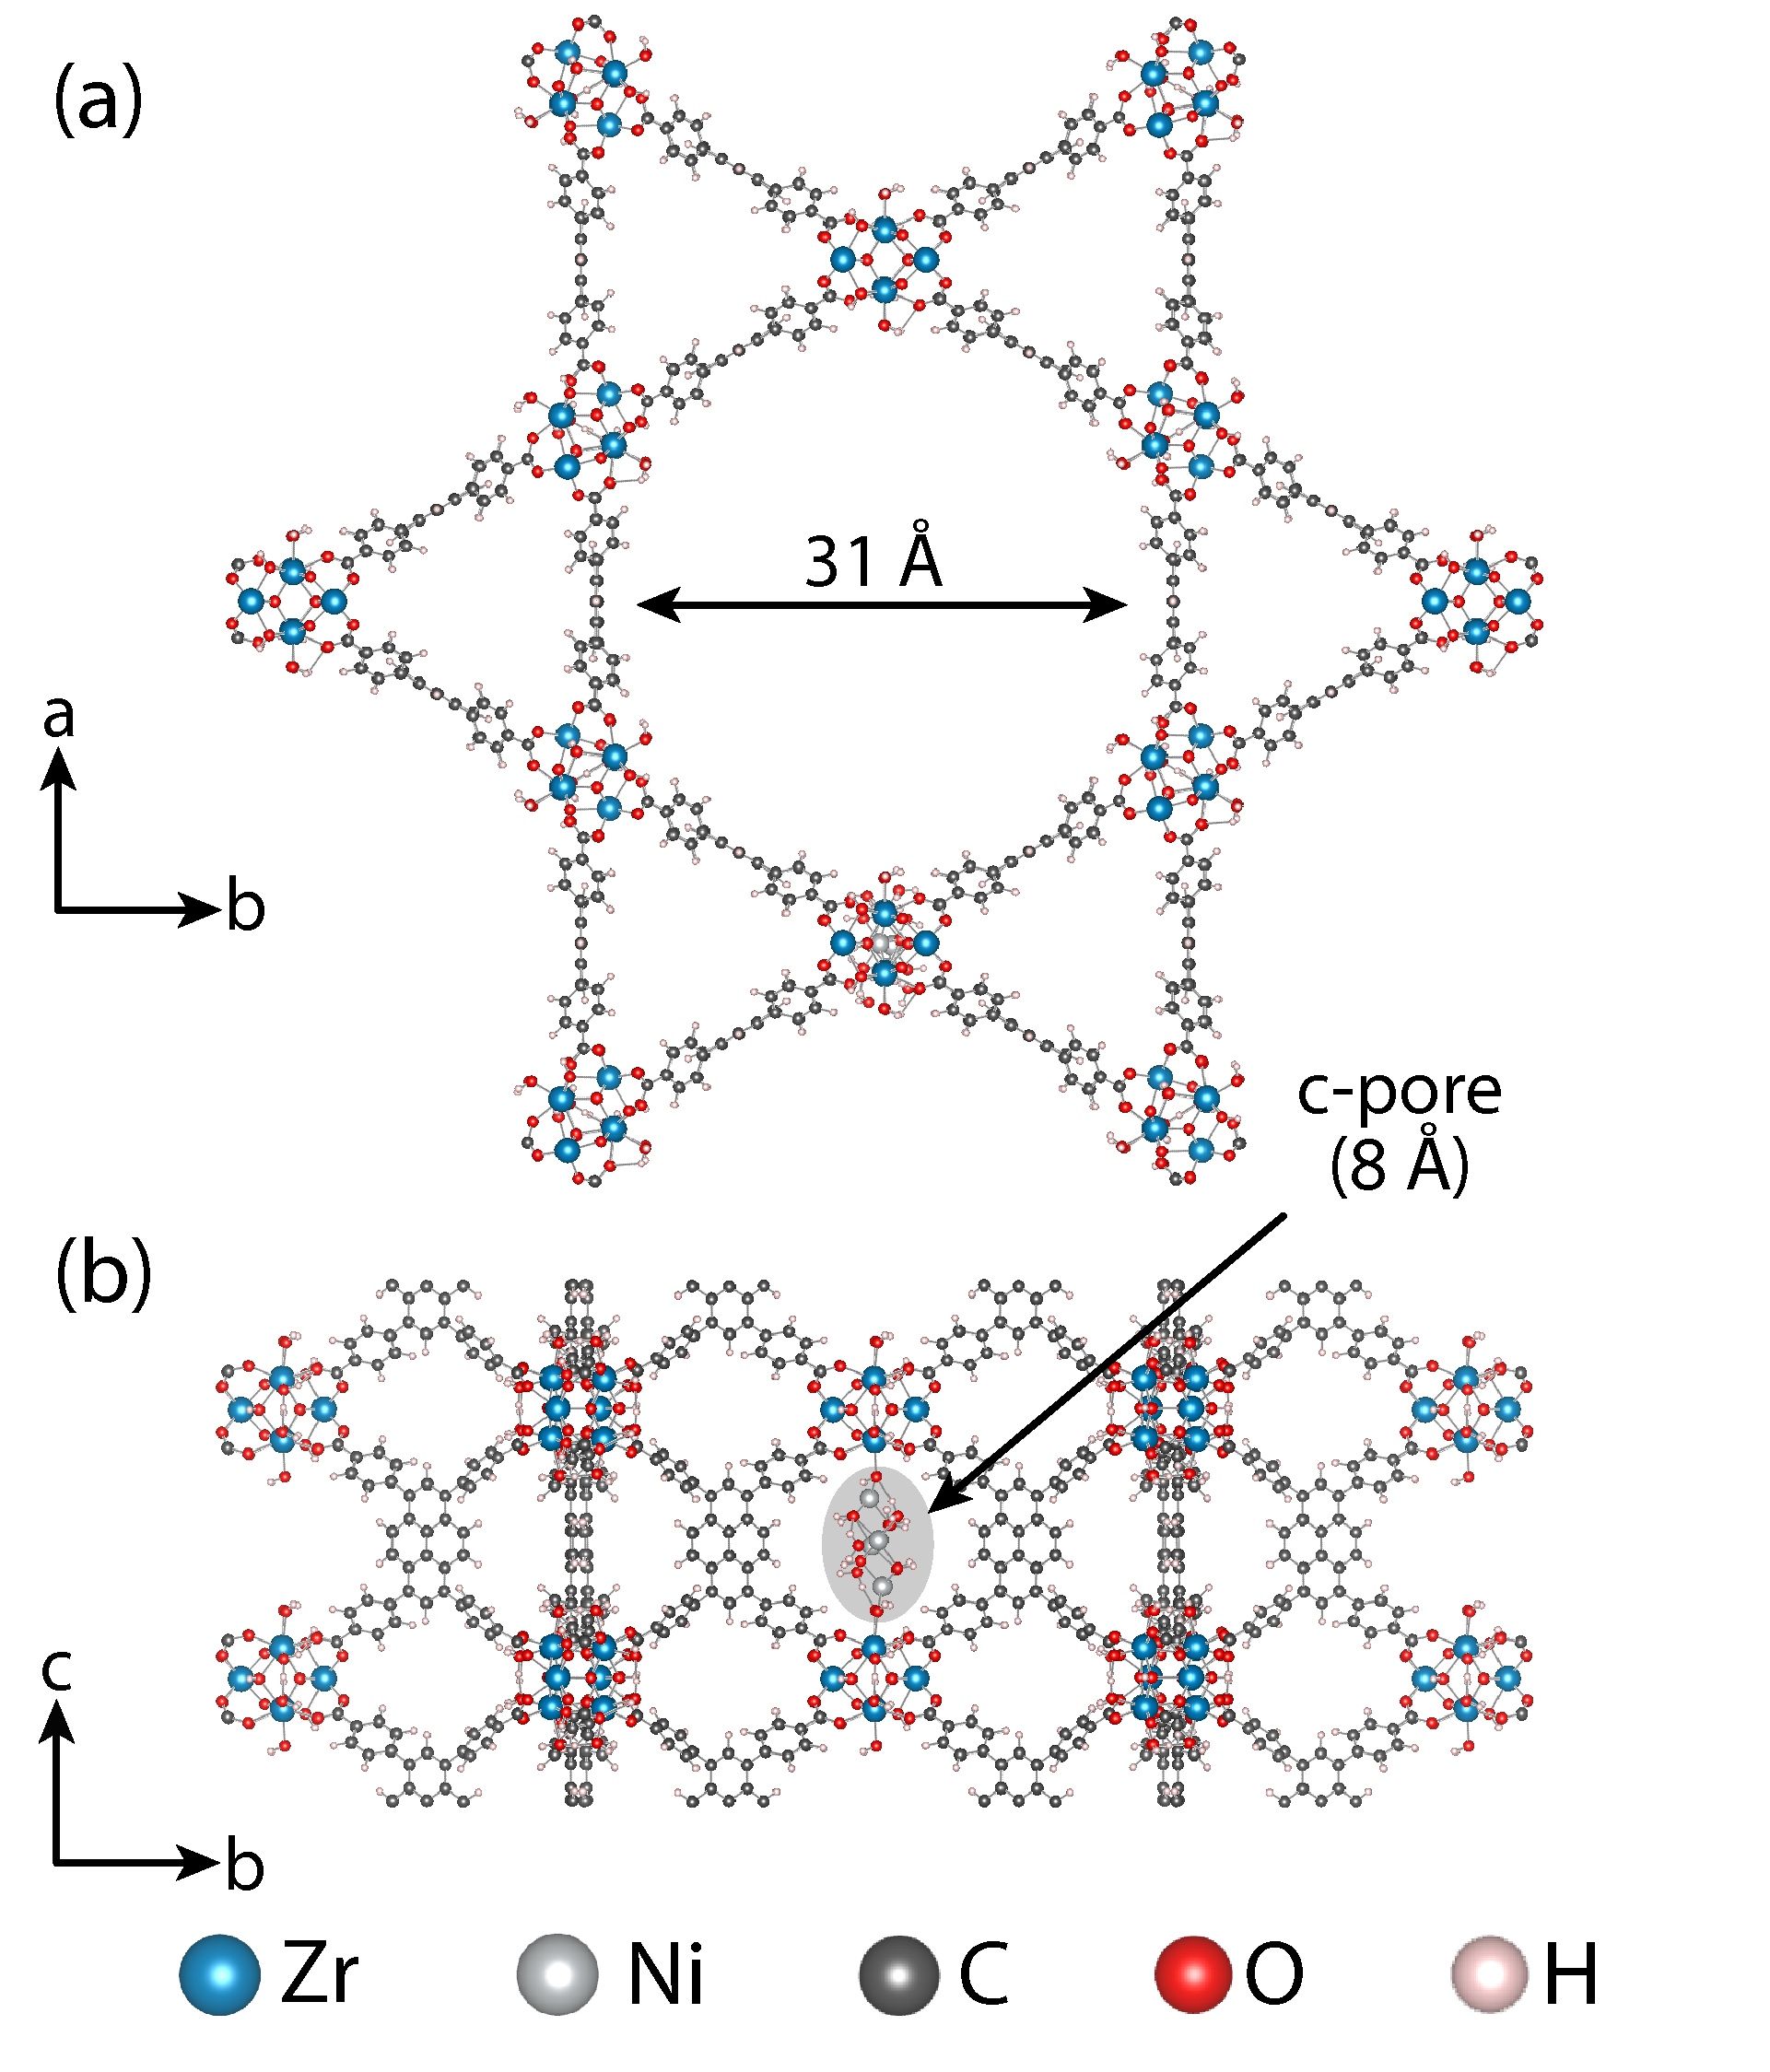
\includegraphics[width=3.0in]{zi-images/00-General-Graphics/2022-figure-MOF-schematic.png}
    \caption{
    The structure of NU-1000 shown along the (a) c-axis and the (b) a-axis with the location of the metal complex location highlighted by the gray oval (shown in  (b)). The \ce{Ni4} cluster spans the length of the c-pore of NU-1000 ($\sim$10 {\AA}), and is attached to adjacent nodes of the pore.
    }
    \label{fig:Ni-MOF-model}
\end{figure}

\subsection{Catalyst Models}

NU-1000 (Figure~\ref{fig:Ni-MOF-model}a) comprises zirconium oxide (\ce{Zr6(\mu_{3}-O)4(\mu_{3}-OH)4(H2O)4(OH)4}) nodes connected by pyrene linker molecules. DFT-optimized unit cell parameters are $a=b=40.611$ {\AA}, $c=15.990$ {\AA}, $\alpha=\beta=\ang{90}$, and $\gamma=\ang{60}$, in agreement with prior work.\cite{PlateroPrats2017} The choice to use a maximum of four \ce{Ni} is based off prior work, with \citeauthor{PlateroPrats2017} revealing the \ce{Ni(II)} cluster most likely consists of four \ce{Ni} atoms from difference envelope density (DED) analysis.\cite{PlateroPrats2017} Catalyst models are constructed within the the 8 {\AA} pore of NU-1000 (Figure~\ref{fig:Ni-MOF-model}b) following prior work.\cite{PlateroPrats2017} Here, the \ce{Ni} clusters attach to NU-1000 by replacing protons on the NU-1000 \ce{Zr} nodes.\cite{Ortuno2016} Catalyst models adopt a variety of ligand environments that include hydroxyl (\ce{OH}), water (\ce{H2O}), hydride (\ce{H}), and oxygen (\ce{O}) ligands, as shown in Figure~\ref{fig:Ni-MOF-structures}. In all, we generated \textbf{\color{red}XXX} structures; \textbf{\color{red}the full library can be accessed on our GitHub page.} 

\begin{figure}[H]
    \centering
    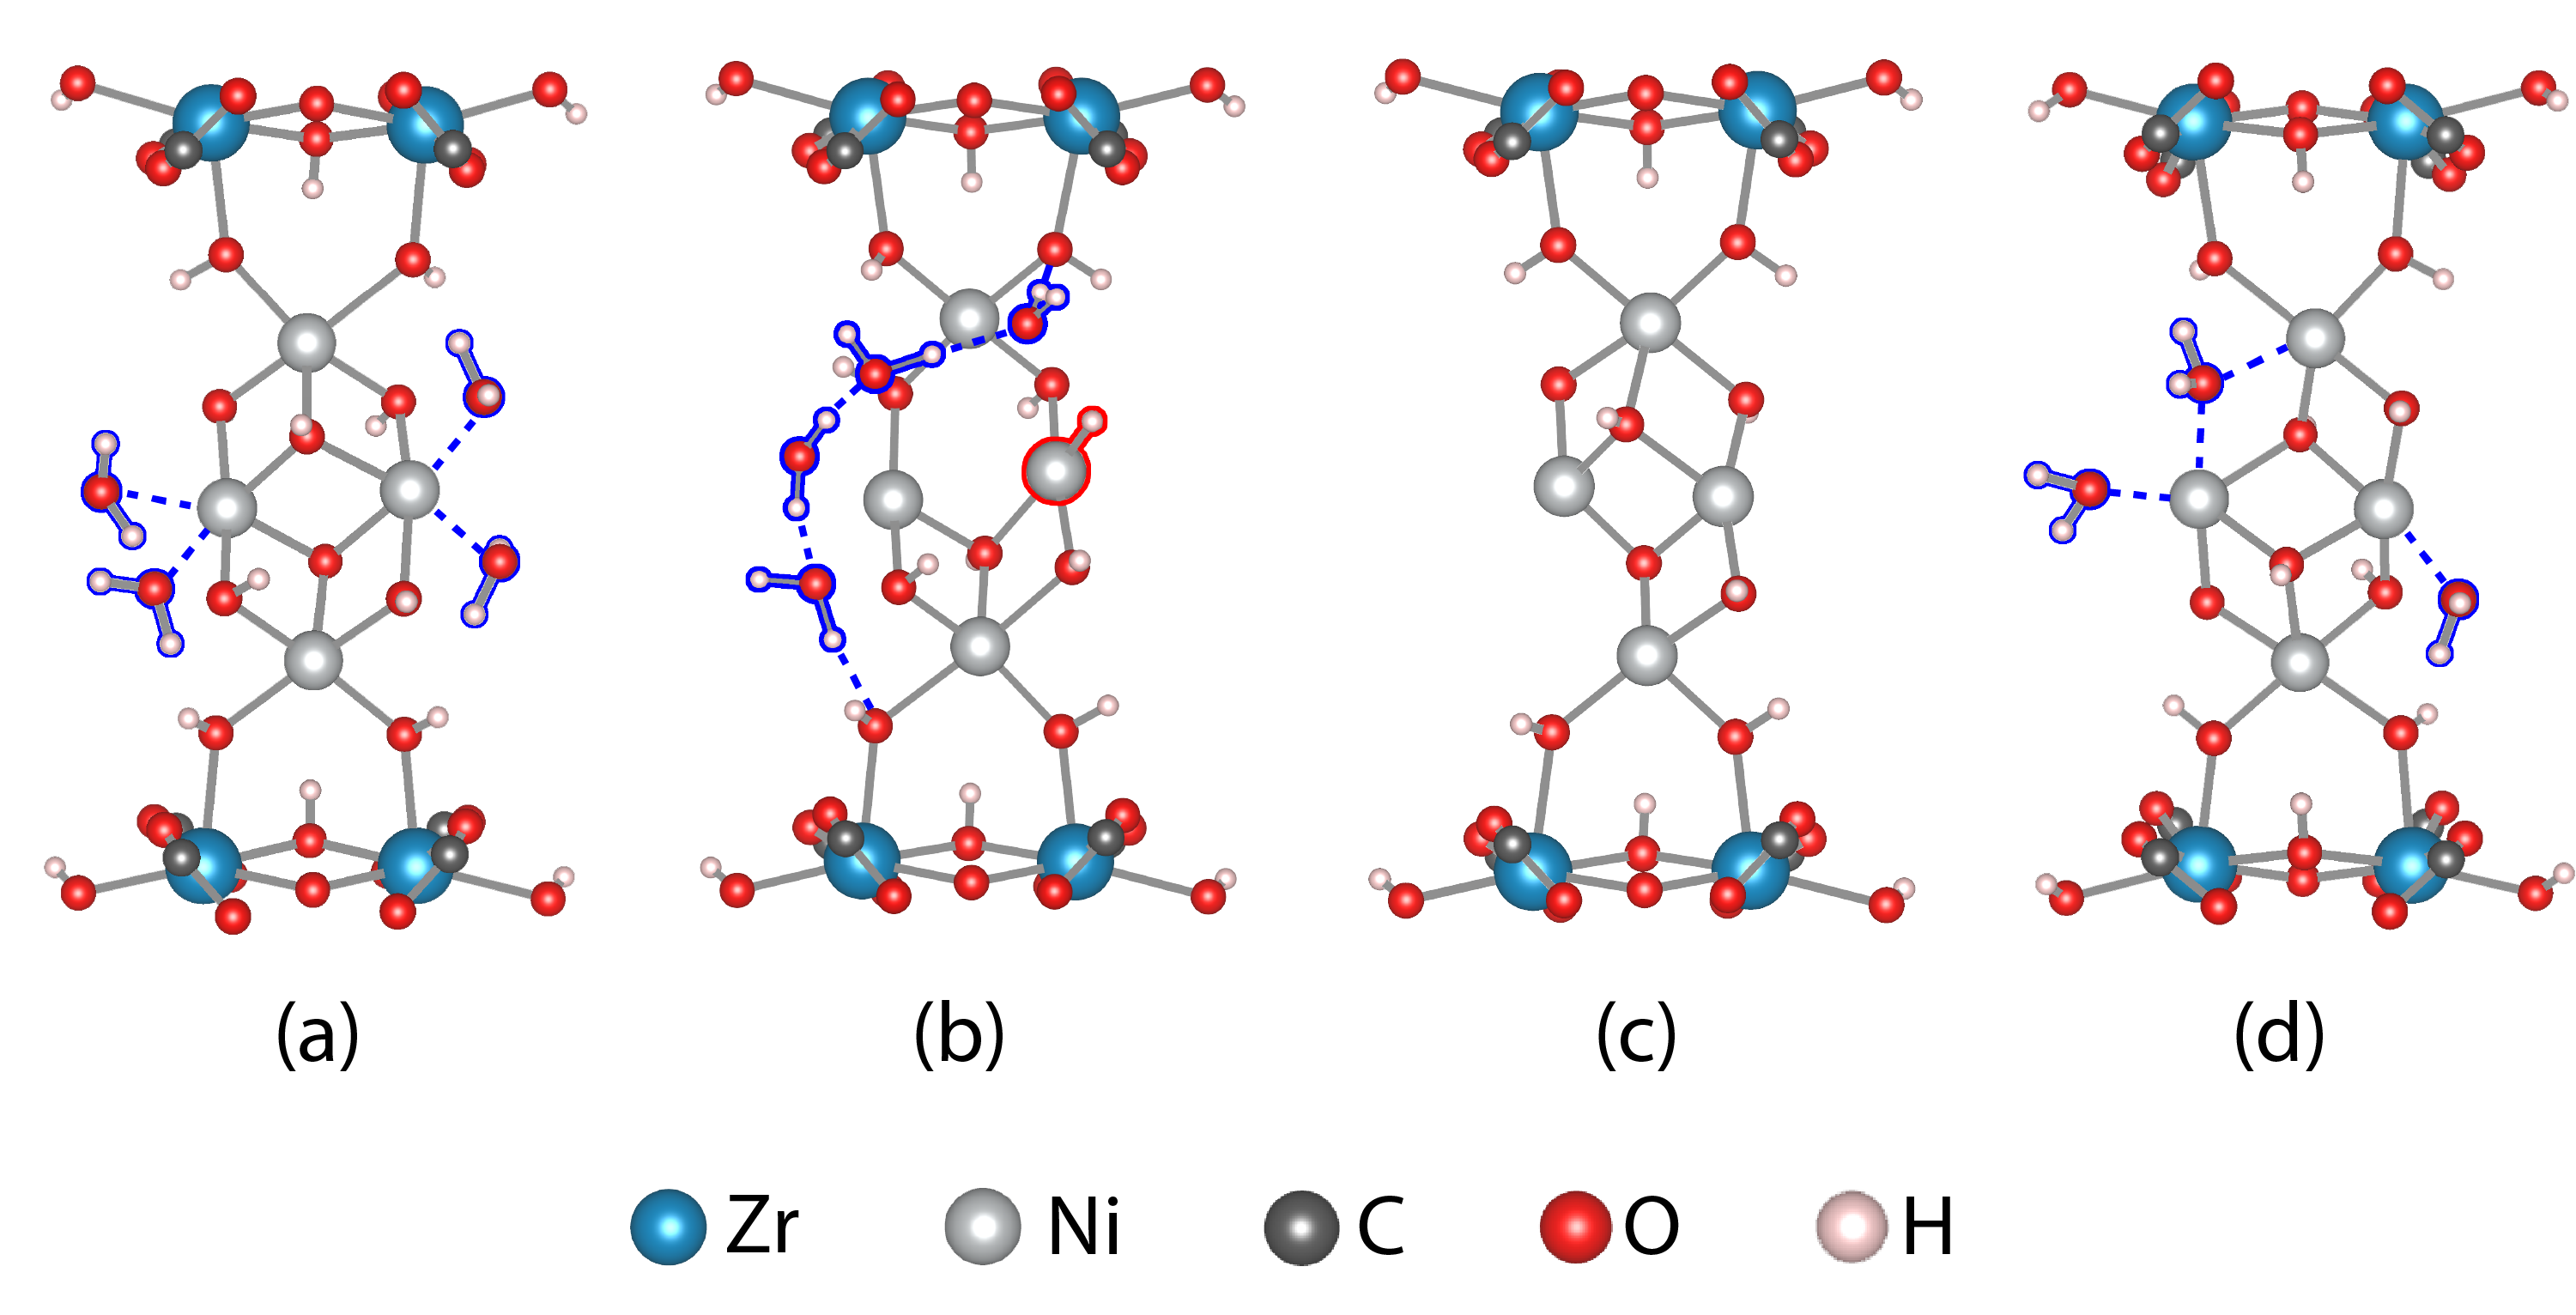
\includegraphics[width=5.0in]{zi-images/00-General-Graphics/2022-figure-clusters-3xstructures.png}
    \caption{
    Different variations of the \ce{Ni} cluster are shown in (a), (b), and (c) with the node of the MOF framework truncated from the renderings. All adsorbed \ce{H2O} molecules are outlined in blue. The diverse ligand \ce{Ni} coordination environments are present with \ce{Ni} coordinating \ce{H2O} and \ce{OH} ligands (all structures), \ce{H} ligands (b), and \ce{O} ligands (c). The reference structure for \textit{ab initio} thermodynamic analysis is shown in (a).
    }
    \label{fig:Ni-MOF-structures}
\end{figure}

\subsection{Differential Pair Distribution Function Analysis}
The pair distribution function (PDF), G(r), represents the local structure as a histogram atom-atom distances in the material weighted by the scattering power of the atoms involved. While the measured PDF reflects all atom-atom distances within the material, by deriving a differential PDF (dPDF), where the PDF measured for NU-1000 is subtracted from the PDF measured for the Ni-complex containing Ni-NU-1000, we analytically isolate the atom-atom distances that define the \ce{Ni} cluster and its interaction with NU-1000 support. Thus the dPDF includes the interatomic distances  within the cluster (\ce{Ni{\Compactcdots}Ni}, \ce{Ni-O}, \ce{O{\Compactcdots}O} atom pairs) and between the cluster and the MOF (\ce{Ni{\Compactcdots}Zr} and \ce{Ni{\Compactcdots}O}) with atom pairs not directly bonded to each other receiving the ``${\Compactcdots}$" notation. PDFs of the computed structural models were simulated within PDFgui using typical values of instrument and atomic displacement parameters for such materials. Given the lower scattering contribution from the \ce{O} atoms compared to \ce{Ni} atoms, \ce{O{\Compactcdots}O} pairs have very low contribution to the measured data and were not calculated. The simulated PDFs were evaluated for their correspondence to the experimental data over XYZ {\AA} range. The experimental details of the PDF measurements are described elsewhere in detail.\cite{PlateroPrats2017} The tetranuclear Nickel cluster exposed to \ce{H2} (3.5\% in \ce{He}) at 200 \degree C for 2 hours and then cooled to 50 \degree C in \ce{H2} for measurement.\cite{PlateroPrats2017} Powder X-ray diffraction (XRD) and total scattering data suitable for PDF analysis were collected at 50 \degree C in \ce{H2}. The dPDFs provide structural insights into the cluster by revealing key interatomic distances with peaks indicating the distance between different atoms. First coordination sphere distances are reported using a line (e.g., \ce{Ni-O}) while second coordination sphere distances are reported using dots (e.g., \ce{Ni{\Compactcdots}Ni} and \ce{Ni{\Compactcdots}Zr}).

\subsection{\textit{ab initio} Thermodynamics Modeling}
The influence of \ce{H2} and \ce{H2O} chemical potentials are explored explored using \textit{ab initio} thermodynamic analysis. In this method, a phase diagram is constructed to report the structures that minimize the free energy in equilibrium with temperatures and pressures in a gas phase reservoir.\cite{Reuter2003,Reuter2004,Grundner2015,Paolucci2016,Li2016,Getman2008,Mandal2020,Zuo2016,Tang2019} The free energy of each \ce{Ni} cluster is calculated as
\begin{equation}
    \begin{split}
        \Delta F^{(2)}(V,T,\mu_{\text{H}},\mu_{\text{OH}},N_{\text{Ni}})  
        & = \Delta F(V,T,N_{\text{H}},N_{\text{OH}},N_{\text{Ni}}) - (\mu_{\text{H}})(\Delta N_{\text{H}}) \\
        & - (\mu_{\text{OH}})(\Delta N_{\text{OH}})  \\ 
    \end{split}
    \label{eq:free-energy-trans}
\end{equation}
where $F$ is the Helmholtz free energy, $V$ is volume, $T$ is temperature, $\mu$ is chemical potential, and $N$ is the number of each type of ligand. The (2) superscript on $F^{(2)}$ indicates the second Legendre transform of $F$,\cite{Alberty1997} i.e., of $N_{\ce{H}}$ and $N_{\ce{OH}}$ to $\mu_{\ce{H}}$ and $\mu_{\ce{OH}}$, respectively. $F$ is equal to $E^\text{elec} + E^\text{ZP} + F^\text{vib}$, where $E^\text{elec}$ is the electronic energy calculated with DFT, $E^\text{ZP}$ is the zero point vibrational energy, and $F^\text{vib}$ is the temperature dependent vibrational free energy. The $\Delta$'s in Eq.~\ref{eq:free-energy-trans} indicate quantities taken relative to a reference structure. The reference structure is defined as a \ce{Ni4(OH)6} cluster with four \ce{H2O} ligands (see supporting information Figure SXXX). Free energies are calculated assuming equilibrium with an \ce{H2} reservoir to simulate conditions commensurate with catalytic hydrogenation, thus enabling different compositions of \ce{H} to be explored. Further, the structure is also assumed to be in equilibrium with an \ce{H2O} reservoir to account for different \ce{O} content of the cluster (in the form of \ce{O}, \ce{OH}, and \ce{H2O} ligands). Following these assumptions, $\mu_{\ce{H}} = 1/2 \mu_{\ce{H}_2(\text{g})}$, $\mu_{\ce{H2O}} = \mu_{\ce{H2O}(\text{g})}$, and $\mu_{\text{OH}} = \mu_{\text{H}_2\text{O}} - \mu_{\text{H}}$. The chemical potentials are calculated as\cite{Grundner2015}

\begin{equation}
    \mu_{\ce{H}_2(\text{g})}(T,P_{\text{H}_{2}}) = E^\text{elec}_{\text{H}_{2}} + E^\text{ZP}_{\text{H}_{2}} + \Delta \mu_{\text{H}_{2}}(T,P_{\text{H}_{2}})
\end{equation}

The \ce{H2O} chemical potential ($\mu_{\ce{H}_2\text{O}(\text{g})}(T,P_{\text{H}_{2}\text{O}})$) is computed analogously as a function of $\Delta \mu_{\text{H}_{2}\text{O}}(T,P_{\text{H}_{2}\text{O}})$. Phase diagrams are constructed in two dimensions as a function of $\Delta \mu_{\text{H}_{2}}(T,P_{\text{H}_{2}})$ and $\Delta \mu_{\text{H}_{2}\text{O}}(T,P_{\text{H}_{2}\text{O}})$ to demonstrate the most thermodynamic favorable compositions of the cluster.

\subsection{Density Functional Theory Calculations}
Electronic energies are calculated using the CP2K software package.\cite{Hutter2014} The exchange correlation energy is calculated with the PBE functional\cite{Perdew1996} and corrected using damped D3 dispersion corrections formulated by \citeauthor{Grimme2010}\cite{Grimme2010} The DZVP-MOLOPT basis set is used to model the valance electrons, and the Goedecker pseudopotentials\cite{Goedecker1996} are used to model the core electrons. The plane wave cutoff energy is 360 Ry. The Unrestricted Kohn-Sham (UKS) method is employed given the open shell natures of the \ce{Ni} ions. For example, a single \ce{Ni(II)} ion can adopt either a singlet or triplet state; therefore, clusters with four \ce{Ni} ions can adopt singlet, triplet, quintet, septet, or nonet states. We consider all possible spin states for \ce{Ni} species for each catalyst composition.\cite{Shabbir2020,Ye2017,Bernales2016,Mandal2020b} Any spin state exhibiting spin contamination is not considered in \textit{ab initio} thermodynamic modeling (see supporting information for more details). The final values of $E$ used in \textit{ab initio} thermodynamic modeling are obtained from geometry relaxations where all atoms in the periodic unit cell are allowed to relax. A sample input file for the CP2K calculations is provided in Supporting Information. Additionally, full descriptions of how $E_{\text{H}_2}$ and $E_{\text{H}_2\text{O}}$ are calculated are provided in Supporting Information.

To compute $E^\text{ZP}$ and $F^\text{vib}$, the vibrational modes are first calculated using the CP2K software package. At each unique composition, we compute the vibrational modes for structures within 100 kJ/mol of lowest energy structure at that configuration, which reduced the number of structures from \hl{XXX} to \hl{XXX} for vibrational mode analysis. We fix the organic linker and inorganic nodes, thereby only calculating only the \ce{Ni} cluster vibrational contributions to the free energy ($F^\text{vib}$). We ensure that the same atoms are fixed across all frequency calculations in order to correctly compare ($F^\text{vib}$). When constructing the vibrational partition function, all frequencies less than 50 cm\textsuperscript{-1} are replaced with 50 cm\textsuperscript{-1} to correct for the breakdown in the harmonic oscillator approximation for low frequency vibrational modes.\cite{Ribeiro2011} The partitions functions are computed in the pMuTT\cite{LYM2019106864} Python package to compute $E^\text{ZP}$ and $F^\text{vib}$ for all structures. A sample input file for the CP2K frequency calculations is provided in the Supporting Information.

\section{Results}
%%%%%%%%%%%%%%%%%%%%%%%%%%%%%%%%%%%%%%%%%%%%%%%%%%%%%%%%%%%%%%%%%%%%%
%% Results 
%%%%%%%%%%%%%%%%%%%%%%%%%%%%%%%%%%%%%%%%%%%%%%%%%%%%%%%%%%%%%%%%%%%%%

% dPDF Diagram
\begin{figure}[H]
    \centering
    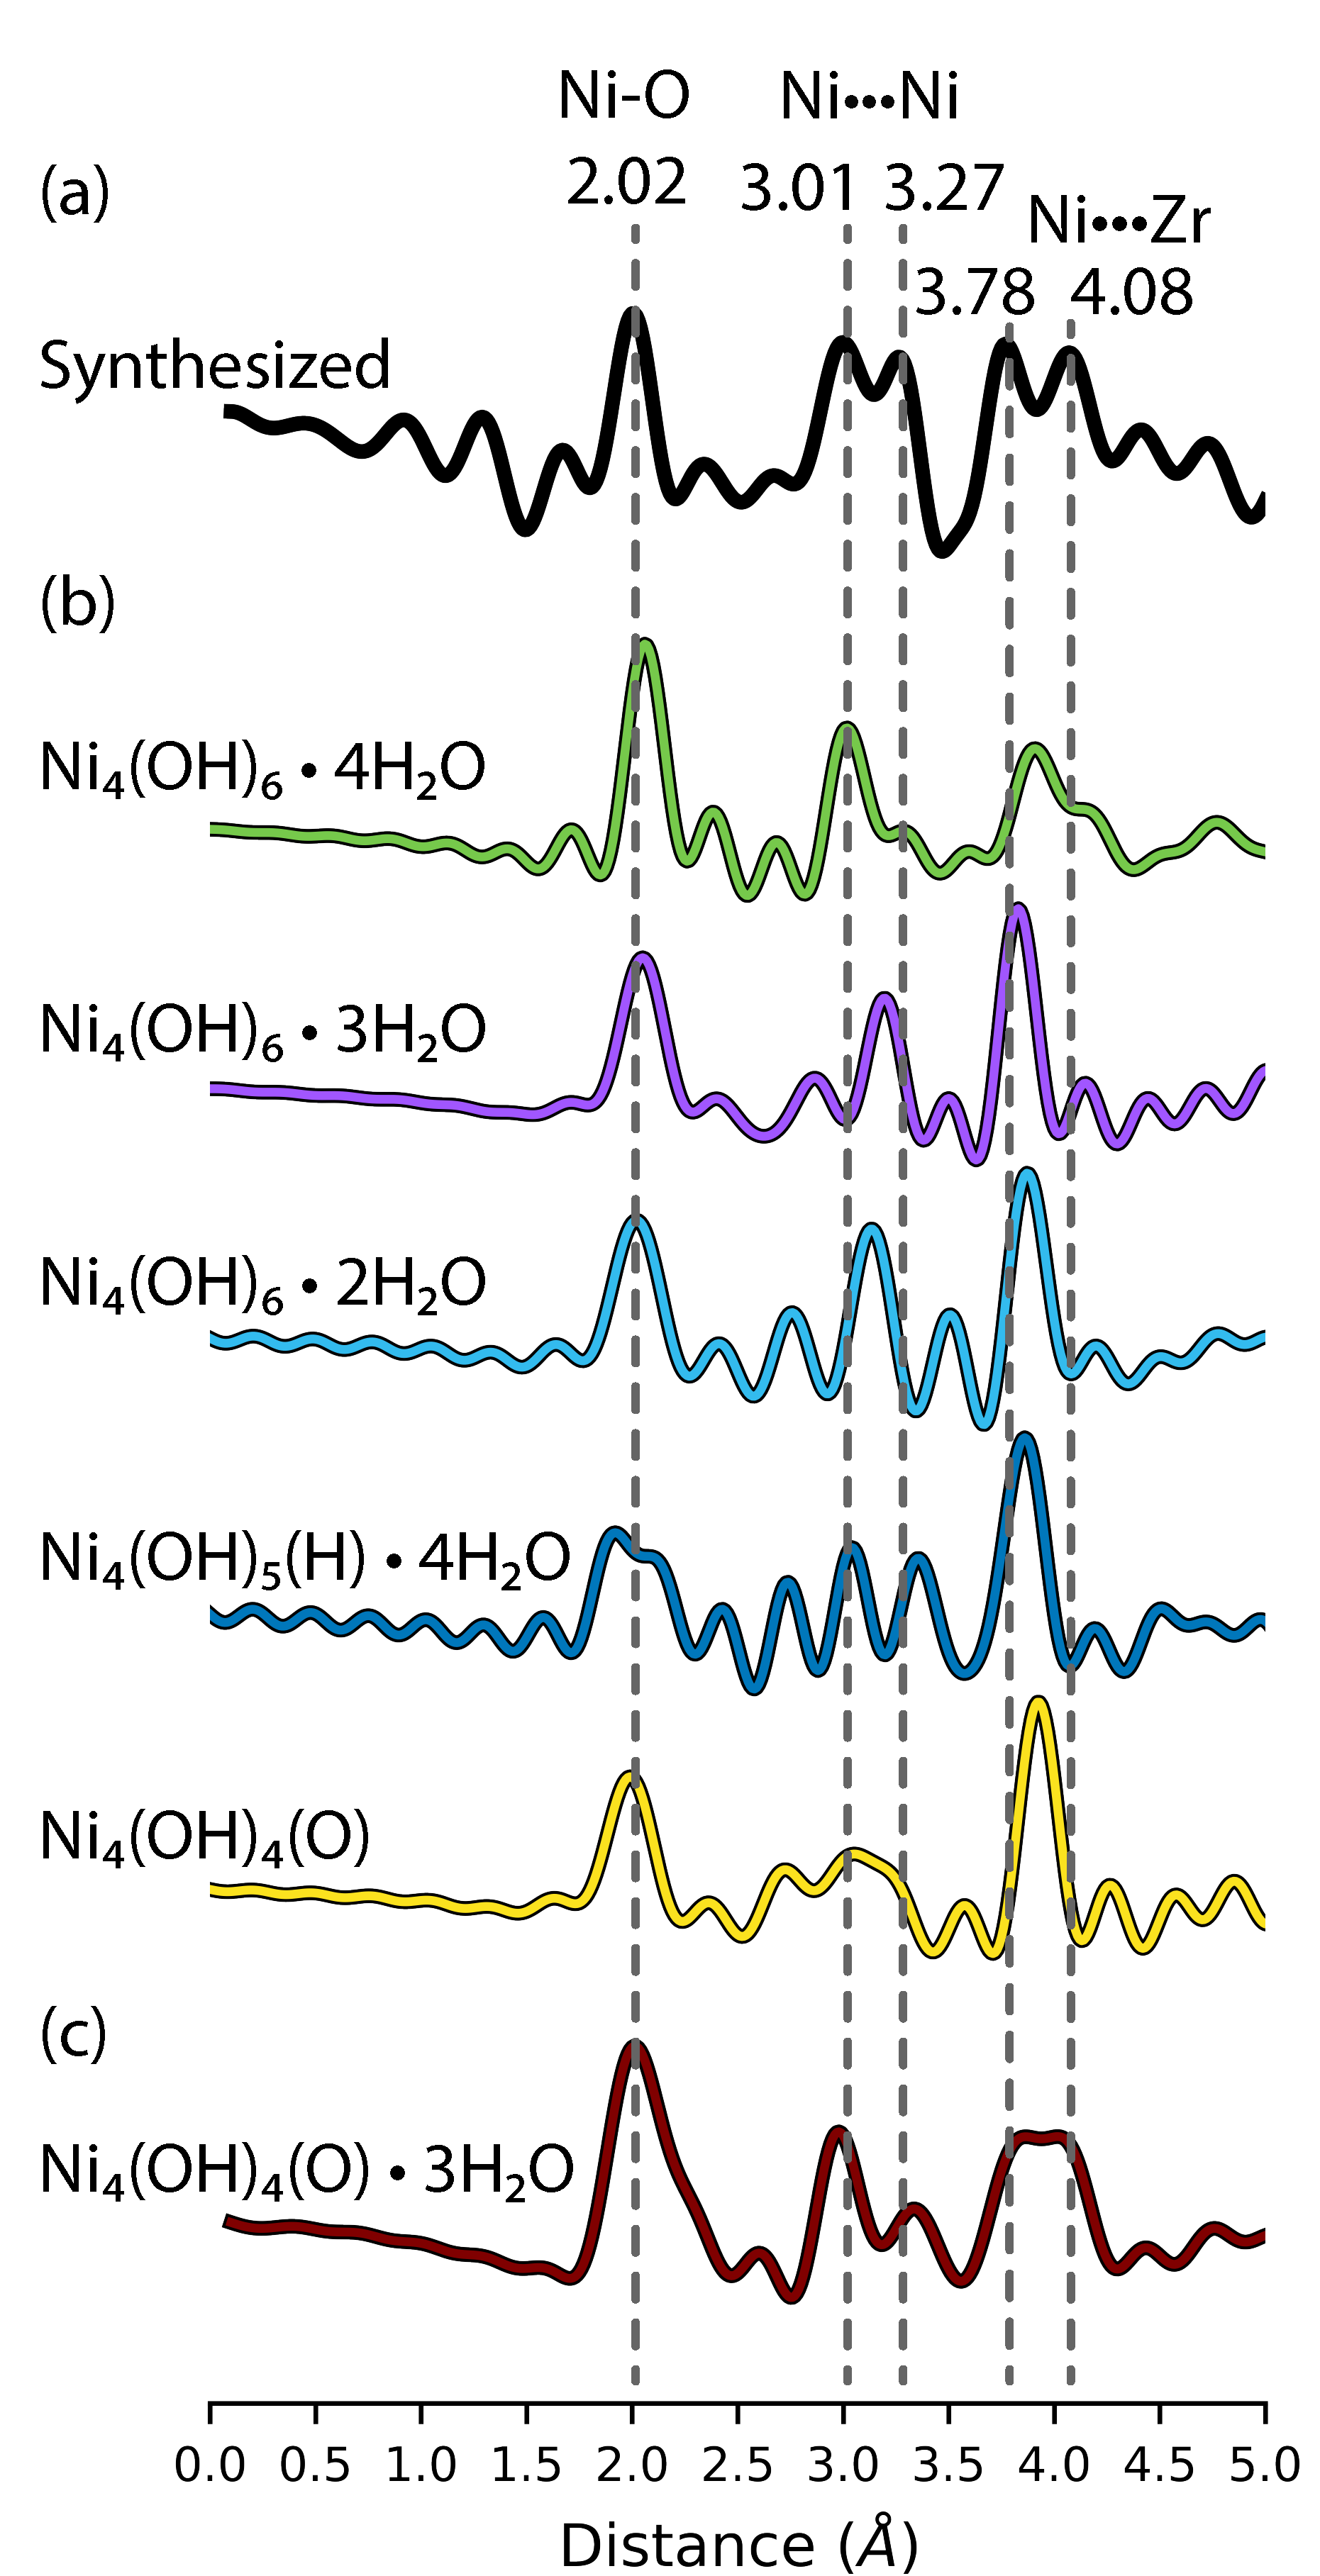
\includegraphics{zi-images/01-Ni-Graphics/2021-MAIN-single-dPDF.png}
    \caption{
    Differential pair distribution functions (dPDFs) capturing the local structural information of the \ce{Ni} cluster. The (a) experimental dPDF, (b) select thermodynamic minima from \textit{ab initio} thermodynamic modeling structures, and (c) a select non-thermodynamic minima structure are reported. The \ce{Ni-O}, \ce{Ni{\Compactcdots}Ni}, and \ce{Ni{\Compactcdots}Zr} distances of the experimental are indicated by the gray dashed lines, enabling comparisons in peak positions between the experimental and model structures. The color scheme is the same as in Figures~\ref{fig:Ni-structure-diagram} and \ref{fig:phase_diagram_Ni}.
    }
    \label{fig:dPDFs-graphic}
\end{figure}

The experimental result from dPDF analysis is shown in Figure~\ref{fig:dPDFs-graphic} (a), where the dPDF of the experimentally observed structure exposed to \ce{H2} gas is depicted. \cite{PlateroPrats2017} From \citeauthor{Ye2017}, the first coordination sphere of the \ce{Ni4} cluster is thought to be comprised of \ce{OH} and \ce{H2O} ligands with \ce{OH} ligands forming links between \ce{Ni} atoms and \ce{H2O} binding on the ``open" sites of the \ce{Ni} ions in the center of the chain.\cite{Ye2017} The atomic composition and arrangement leads to differences in peak position and width in the dPDF measurements. Key peaks in the experimentally observed dPDF are the single peak at 2.02 {\AA}, split peaks at 3.01 {\AA} and 3.27 {\AA}, and split peaks at 3.78 {\AA} and 4.08 {\AA} (Figure~\ref{fig:dPDFs-graphic} (a)). These correspond to \ce{Ni-O}, \ce{Ni{\Compactcdots}Ni}, and \ce{Ni{\Compactcdots}Zr} distances, respectively. Our analysis primarily focuses on the \ce{Ni-O} and \ce{Ni{\Compactcdots}Ni} seen in the experimental dPDF. We compare the peak positions of model structures (Figure~\ref{fig:dPDFs-graphic} (b) and (c)) to the peak positions of the experimental dPDF (Figure~\ref{fig:dPDFs-graphic} (a)). 

% Structure Diagram
\begin{figure}[H]
    \centering
    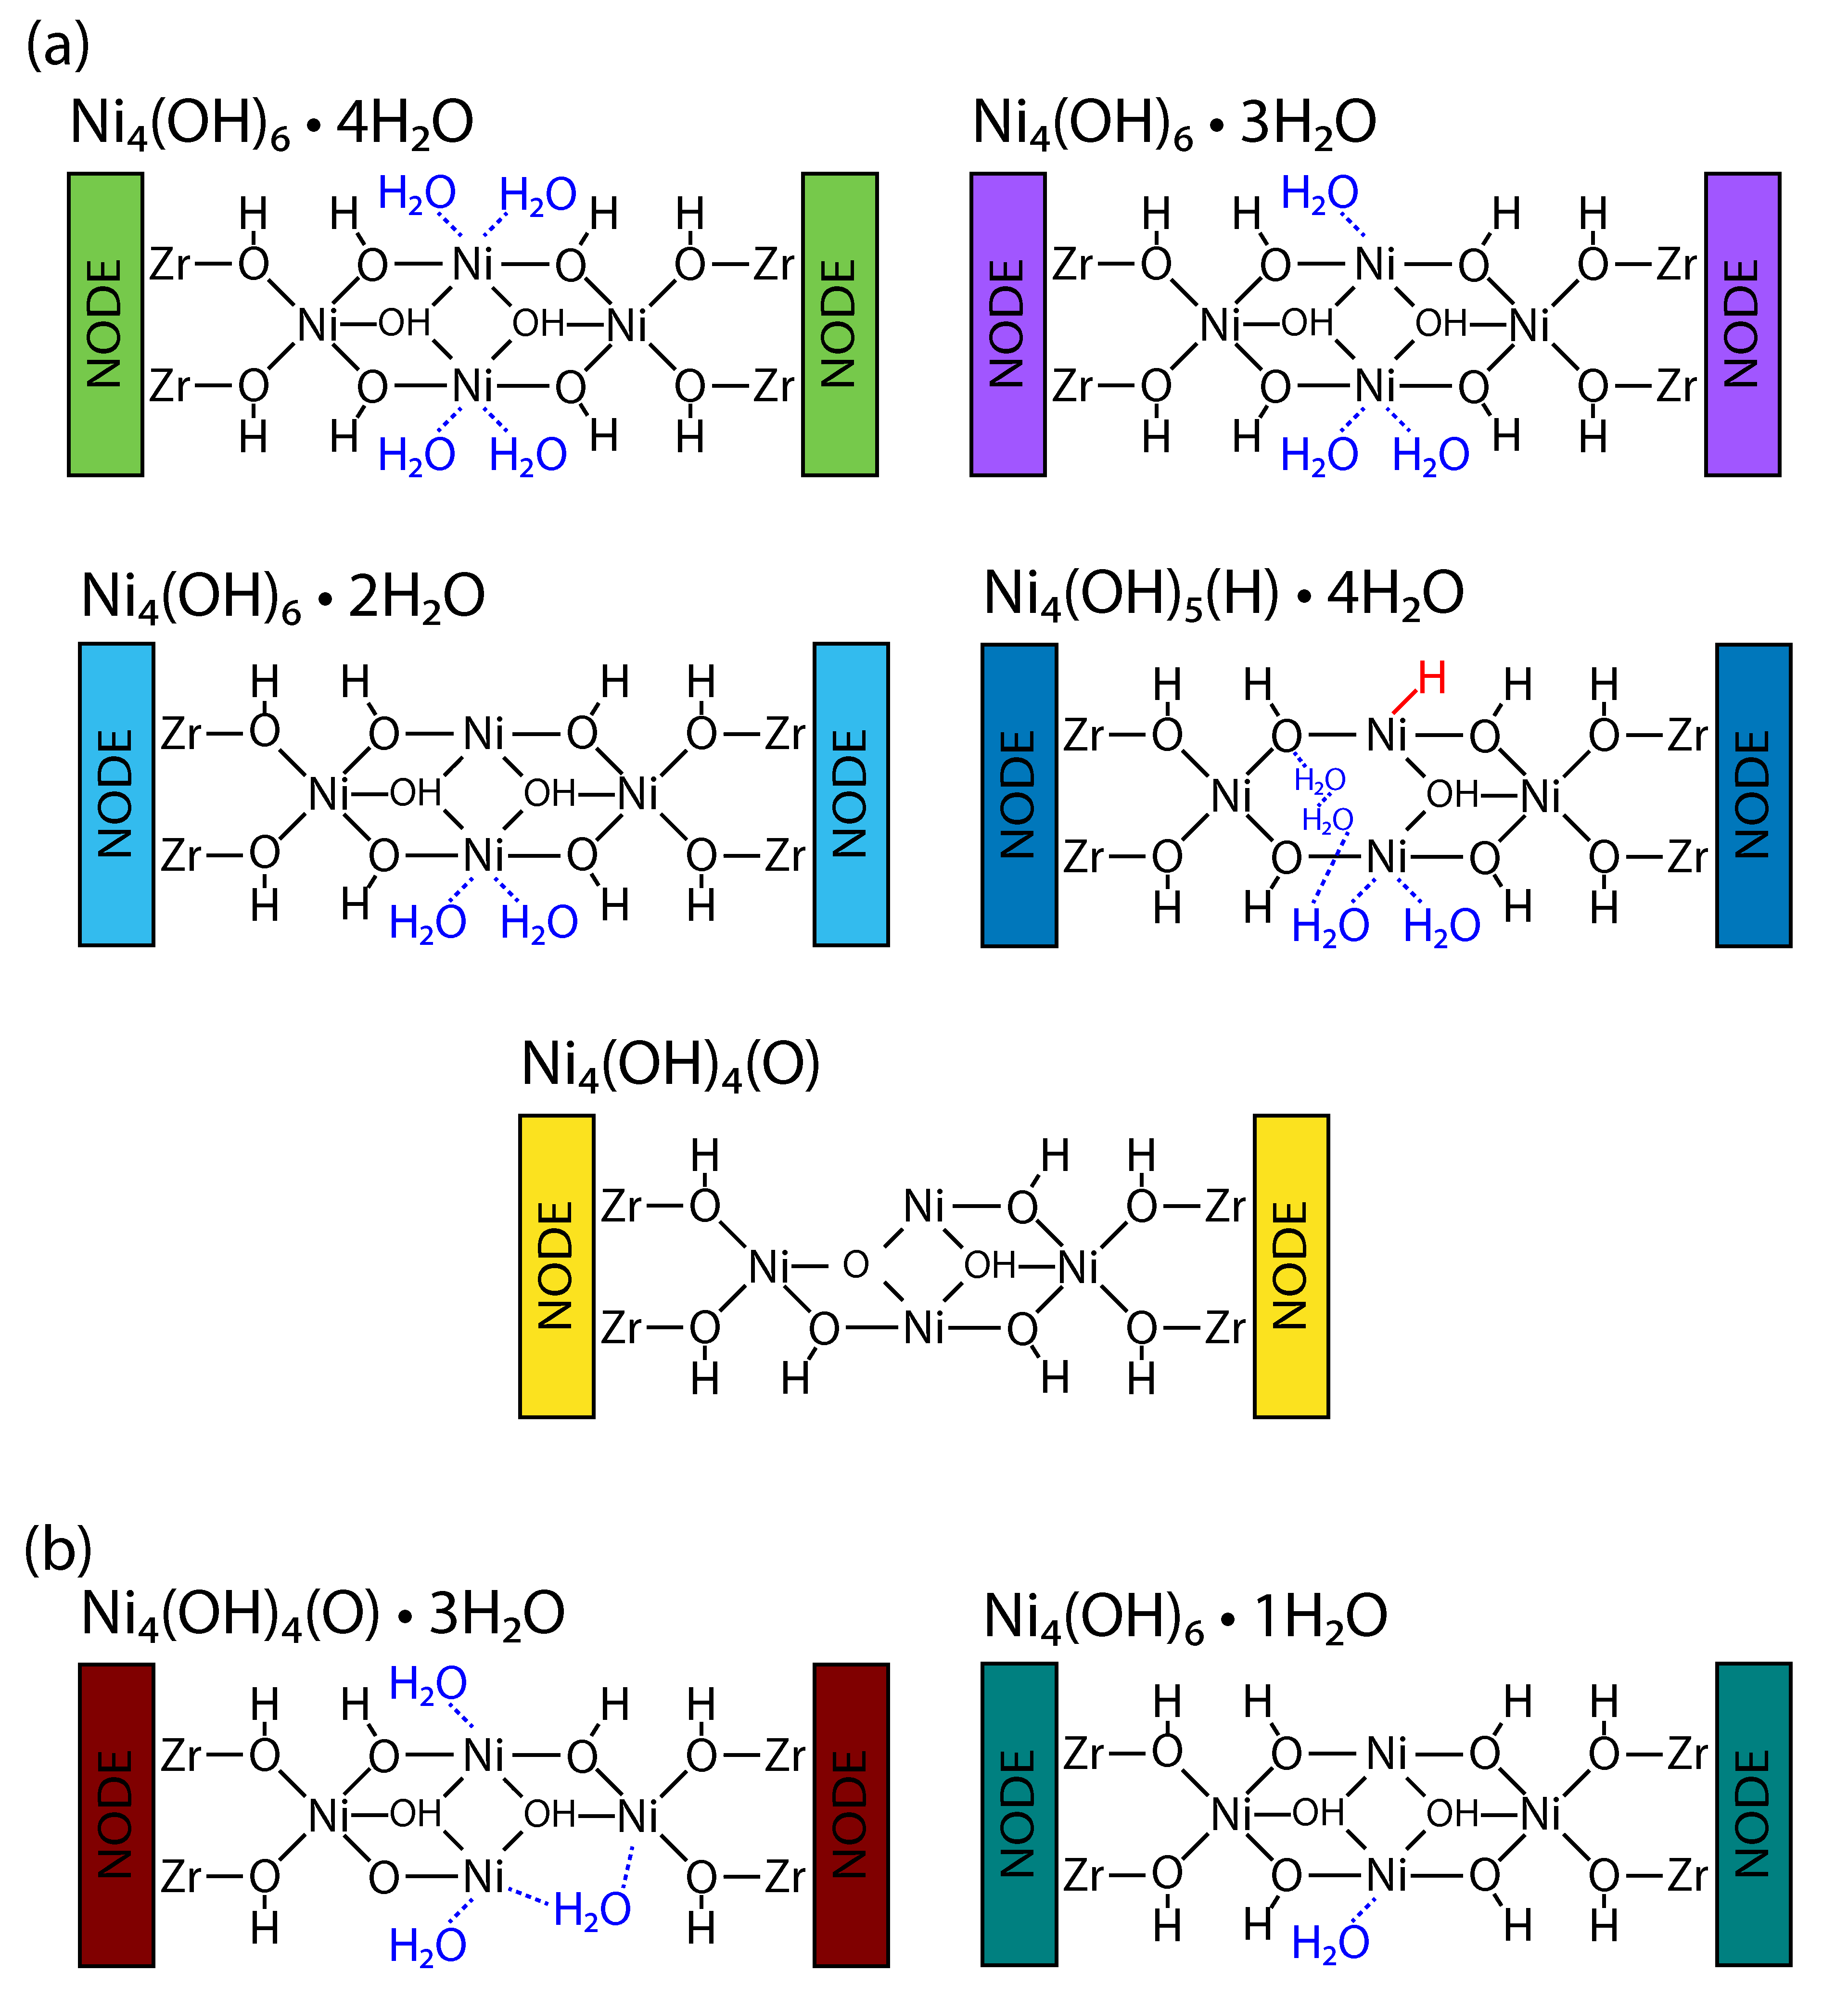
\includegraphics[width=0.75\textwidth]{zi-images/01-Ni-Graphics/2021-MAIN-structure-diagram.png}
    \caption{
    Depiction of key structures considered in this work from (a) \textit{ab initio} thermodynamic modeling structures and (b) select non-thermodynamic minima. The color scheme is the same as in Figures~\ref{fig:phase_diagram_Ni} and \ref{fig:dPDFs-graphic}. All \ce{H2O}s are colored blue, and any Nickel hydride species (\ce{Ni-H}) are colored red. The color scheme is the same as in Figures~\ref{fig:phase_diagram_Ni} and \ref{fig:dPDFs-graphic}.
    }
    \label{fig:Ni-structure-diagram}
\end{figure}

% paragraph on the structure with good coordination from the structure diagrams
Furthermore, the \ce{Ni-O} coordination number of the activated structure is measured to be $\sim$5 when exposed to \ce{H2} gas. We use the following information as a reference during \textit{ab initio} thermodynamic analysis to identify appropriate \ce{H2} and \ce{H2O} chemical potential values. We neglect \ce{Ni-O} coordination numbers below 3.3 because the lack of \ce{Ni-O} coordination suggests these aren't relevant structures, which is confirmed by their dPDFs (\hl{see Supporting Information}). All structures appearing on the phase diagram (Figure~\ref{fig:phase_diagram_Ni}) are located within the \hl{Supporting Information.} The structures from \textit{ab initio} thermodynamic analysis that minimize the free energy expression (Eq. \ref{eq:free-energy-trans}) and exhibit \ce{Ni-O} coordination numbers above 3.3 are shown in Figure~\ref{fig:Ni-structure-diagram} (a). We order the structures according to the \ce{Ni-O} coordination numbers, determined by inspecting the \ce{Ni-O} bond distances within each structure. The exact \ce{Ni-O} coordination numbers are reported on Figure~\ref{fig:phase_diagram_Ni}.

% paragraph about the structures 
The structures with \ce{Ni-O} coordination above 3.3, ranked from highest to lowest, are structures \ce{Ni4(OH)6.4H2O} (green), \ce{Ni4(OH)6.3H2O} (purple), \ce{Ni4(OH)6.2H2O} (cyan), \ce{Ni4(OH)5(H).4H2O} (blue), \ce{Ni4(OH)4(O)} (yellow), and \ce{Ni4(OH)4.2H2O} (orange). The specific \ce{Ni} ligand environments are presented in Figure~\ref{fig:Ni-structure-diagram} (a), with structures exhibiting different \ce{Ni-O} coordination environments. The structures exhibit different compositions featuring \ce{OH}, \ce{H2O}, \ce{H}, and \ce{O} ligands coordinated to the \ce{Ni} atoms. Structures \ce{Ni4(OH)6.4H2O} (green), \ce{Ni4(OH)6.3H2O} (purple), and \ce{Ni4(OH)6.2H2O} (cyan) are the same base \ce{Ni4(OH)6} structure, but contain different \ce{H2O} content (Figure~\ref{fig:Ni-structure-diagram} (a)). Structure \ce{Ni4(OH)5(H).4H2O} (blue) is unique in that it contains both a Nickel-hydride (\ce{Ni-H}) and a bridge of hydrogen bonded \ce{H2O}s. Structure \ce{Ni4(OH)4(O)} (yellow) is the only structure featuring an \ce{O} ligand on the phase diagram, and structure \ce{Ni4(OH)4.2H2O} (orange) features a loss of \ce{OH} ligands coordinated to three different \ce{Ni} atoms. The diverse ligand coordination environment for \ce{Ni} is captured by the structures appearing on the phase diagram (Figure~\ref{fig:phase_diagram_Ni}). 

% Phase Diagram
\begin{figure}[H]
    \centering
    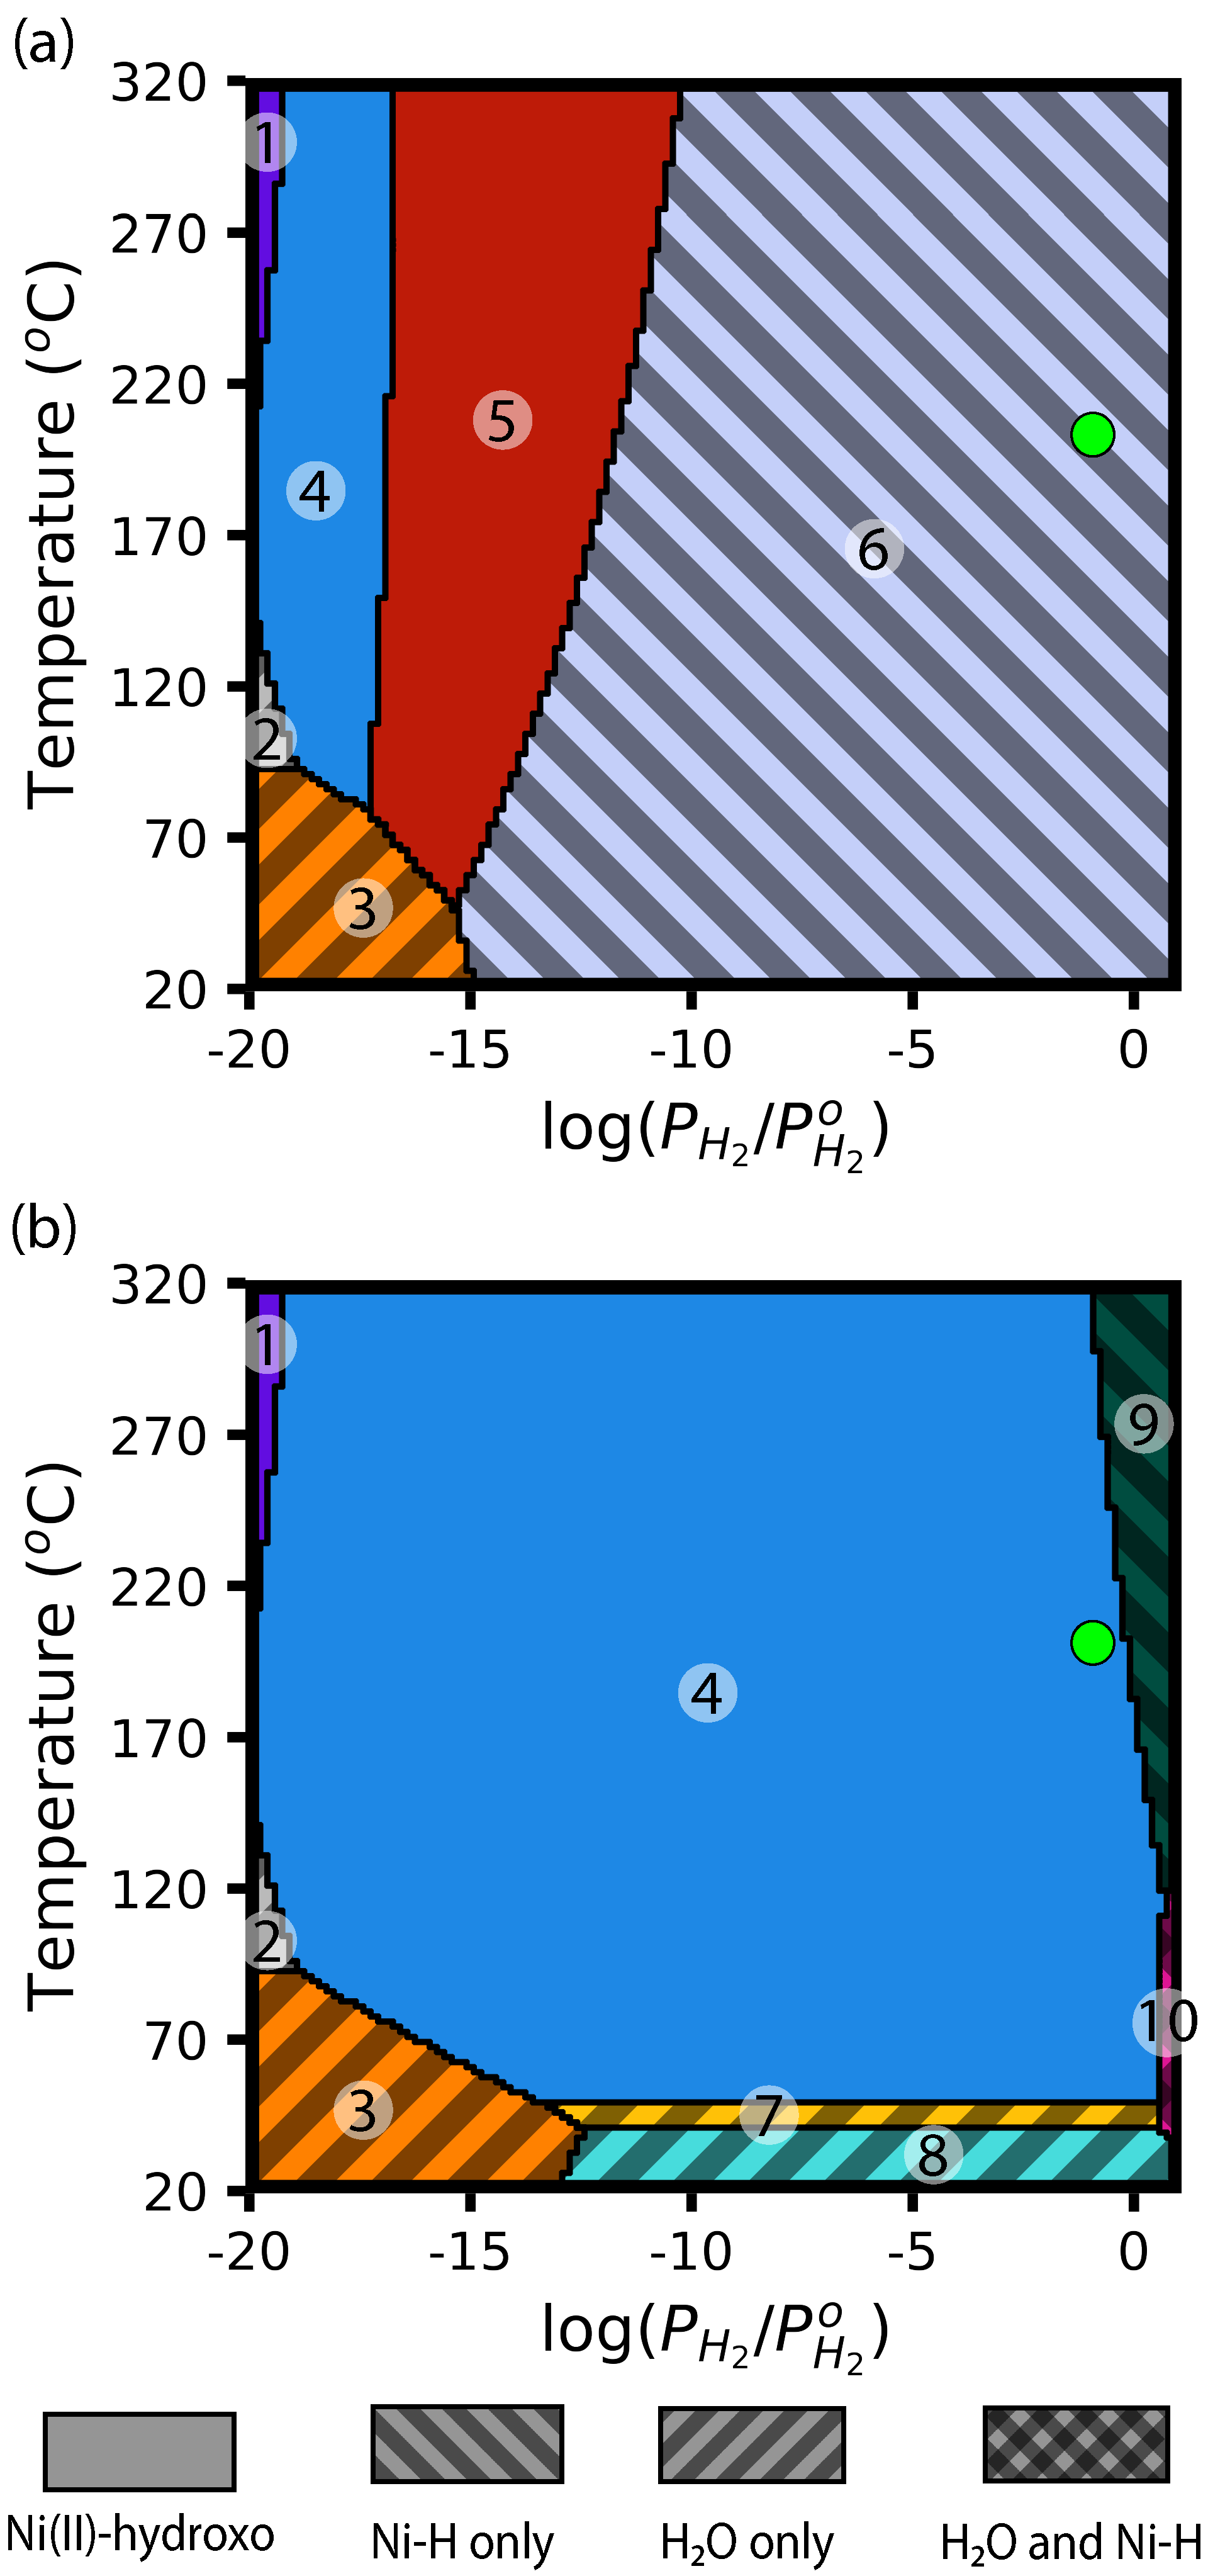
\includegraphics{zi-images/01-Ni-Graphics/2021-MAIN-phase-diagram-combined.png}
    \caption{
    Phase diagram for the \ce{Ni} cluster calculated as a function of $\Delta \mu_{\text{H}_{2}}(T,P_{\text{H}_{2}})$ and $\Delta \mu_{\text{H}_{2}\text{O}}(T,P_{\text{H}_{2}\text{O}})$. The different structures are represented by the different colored regions, with follow the same color scheme as previous figures. We are unable to define specific \ce{H2O} conditions for the system; therefore, the white dashed line represents the chemical potential for experimental conditions containing \ce{H2} (3.5\% in \ce{He}) at 50 \degree C. 
    }
    \label{fig:phase_diagram_Ni}
\end{figure}  

% Paragraph on the phase diagram here with the structures with reasonable coordination
We provide insights into the relative stability of structures and compositions from Figure~\ref{fig:Ni-structure-diagram} by constructing phase diagrams as a function of \ce{H2} and \ce{H2O} chemical potential terms. A more positive chemical potential term indicates a higher gas phase chemical potential (i.e., a higher gas phase concentration). The structures on the phase diagrams minimize $F^{(2)}$ at the specified \ce{H2} and \ce{H2O} chemical potentials. Generally, higher \ce{H2O} chemical potential indicates higher \ce{Ni-O} coordination. At lower \ce{H2O} chemical potential (i.e., absence of gaseous \ce{H2O}), a higher \ce{H2} chemical potential indicates reduced \ce{Ni-O} coordination. The \ce{H2} chemical potential suggests the conversion of \ce{OH} ligands into \ce{H2O} ligands that are then driven off the \ce{Ni} cluster. Of interest is the catalyst composition and structure under operating conditions. The precise \ce{H2O} chemical potential within the MOF is undefined; therefore, the catalyst composition and structure under operating conditions is represented by a vertical dashed white line in Figure~\ref{fig:phase_diagram_Ni}. The \ce{H2} chemical potential is computed at experimental conditions containing \ce{H2} (3.5\% in \ce{He}) at 50 \degree C. At more positive \ce{H2O} chemical potentials, we observe structures (Figure~\ref{fig:Ni-structure-diagram} (a)) with coordination numbers much closer to those observed experimentally, which implies the \ce{H2O} chemical potential within NU-1000 is higher than previously thought. Further insights into the structures are provided by dPDF analysis. 

% paragraph talking about the dPDF of the structures on the phase diagram with higher coordination
Our analysis primarily focuses on the \ce{Ni-O} and \ce{Ni{\Compactcdots}Ni} seen in the experimental dPDF (Figure~\ref{fig:dPDFs-graphic} (a)), where we compare the structures with coordination above 4.0 shown in Figure~\ref{fig:dPDFs-graphic} (b). Selecting high \ce{Ni-O} coordination is valid, given the mismatch in peak characteristics for 
structures with low \ce{Ni-O} (\hl{see Supporting Information}). We observe large deviations in peak positions for both the \ce{Ni-O} peak and the split \ce{Ni{\Compactcdots}Ni} peaks at low coordination. As expected, we observe much better agreement between model structures and the experimental dPDF with structures that feature higher \ce{Ni} coordination. 

For the \ce{Ni-O} peak, reasonable agreement by all structures in Figure~\ref{fig:dPDFs-graphic} is seen with the exception of \ce{Ni4(OH)5(H).4H2O} (blue). Rather than a single \ce{Ni-O} peak, \ce{Ni4(OH)5(H).4H2O} (blue) exhibits two peaks centered around the experimental \ce{Ni-O} peak, suggesting the presence of asymmetric \ce{Ni-O} distances within the structure from the bridge of hydrogen bonded \ce{H2O}s within the structure. Given the \ce{Ni-O} peak corresponds to the bond between \ce{Ni} and \ce{O}, major deviations in the \ce{Ni-O} peak (as seen by structures with low coordination) indicates a significant deviation between the \ce{Ni-O} coordination environment of the experimental and model structures. 

There is less agreement for the \ce{Ni{\Compactcdots}Ni} peaks while comparing the experimental and model structures (Figure~\ref{fig:Ni-structure-diagram} (a)). Structures \ce{Ni4(OH)6.4H2O} (green), \ce{Ni4(OH)6.3H2O} (purple), and \ce{Ni4(OH)6.2H2O} (cyan) exhibit a single \ce{Ni{\Compactcdots}Ni} peak within the regime of the experimental split \ce{Ni{\Compactcdots}Ni} peaks. Structure \ce{Ni4(OH)4(O)} (yellow), with the \ce{O} ligand coordinating two \ce{Ni} atoms, lacks a prominent \ce{Ni{\Compactcdots}Ni} peak; a broad peak is observed within the experimental regime. The only structure exhibiting split \ce{Ni{\Compactcdots}Ni} peaks is structure \ce{Ni4(OH)5(H).4H2O} (blue), which again features the Nickel-hydride (\ce{Ni-H}) and a bridge of hydrogen bonded \ce{H2O}s. However, only one of these peaks aligns with the experimental peak. The other peak is observed at a larger distance. 

% Paragraph talking about the asymmetry in ligand environment
A closer inspection of the split peaks in the experimental dPDF at 3.01 {\AA} and 3.27 {\AA} suggests asymmetry in the \ce{Ni} coordination environments. Most structures appearing on the phase diagram (Figure~\ref{fig:phase_diagram_Ni}) are symmetric in their ligand coordination (as showed by the structures located in Figure~\ref{fig:Ni-structure-diagram} (b)). The symmetry in the ligand environment results in symmetric interatomic distances between the different \ce{Ni} species, thereby leading to single peaks \ce{Ni{\Compactcdots}Ni} instead of multiple \ce{Ni{\Compactcdots}Ni} in the 3.01 {\AA} and 3.27 {\AA} range. Our library included structure with asymmetric \ce{Ni} coordination (\hl{as shown in the Supporting information}; however, these structures were not thermodynamic mimima under any explored conditions in \textit{ab initio} thermodynamic analysis. 

% Paragraph about the dPDF of selected structure
Continuing with this idea, we evaluate all structures in our structure library to identify structures that might show better agreement of the \ce{Ni-O} peak and \ce{Ni{\Compactcdots}Ni} split peaks of the experimental dPDF. One such structure is \ce{Ni4(OH)4)(O).3H2O} (red) (shown in Figures~\ref{fig:dPDFs-graphic} (c) and \ref{fig:Ni-structure-diagram} (b)). Structure \ce{Ni4(OH)4)(O).3H2O} (red) is not a thermodynamic minimum under any of the explored conditions, hence why it does not appear on Figure~\ref{fig:phase_diagram_Ni}. This structure exhibits a broad \ce{Ni-O} peak that agrees with the experimental dPDF and split \ce{Ni{\Compactcdots}Ni} peaks that show reasonable agreement. The structure displays a mixture of \ce{OH}, \ce{H2O}, and \ce{O} ligands, and high \ce{Ni} coordination as shown in Figure~\ref{fig:Ni-structure-diagram}. This asymmetric ligand environment breaks the symmetry of coordination, leading to the split to the split \ce{Ni{\Compactcdots}Ni} peaks at distances that closely reasonable those seen in the experimental dPDFs. We observe similar asymmetries in other structures (\hl{see Supporting information}) that show good agreement with the \ce{Ni-O} and \ce{Ni{\Compactcdots}Ni} peaks positions \hl{(see Supporting Information)}. The observed asymmetries include both diversity in the \ce{Ni} coordination environment (\ce{OH}, \ce{H2O}, \ce{O}) as well as the orientation of certain ligands (mainly, \ce{H2O}). 

% Paragraph talking about the Ni...Zr split peaks
The last remaining feature of the dPDFs not explored are the \ce{Ni{\Compactcdots}Zr} split peaks seen in the 3.78 {\AA} and 4.08 {\AA} range in the experimental dPDF (Figure~\ref{fig:dPDFs-graphic} (b)). Similar to the \ce{Ni{\Compactcdots}Ni} split peaks, most structures on the phase diagram (Figure~\ref{fig:phase_diagram_Ni} exhibit a single peak within the experimental range of the \ce{Ni{\Compactcdots}Zr} peaks. Even structure \ce{Ni4(OH)4)(O).3H2O} (red) fails to create the split \ce{Ni{\Compactcdots}Zr} peaks, although this structure does exhibit a broad \ce{Ni{\Compactcdots}Zr} peaks. The \ce{Ni{\Compactcdots}Zr} distance within the MOF is from the attachment of the Nickel SSHC to the MOF node. The \ce{Ni} atoms are connected to the \ce{Zr} via \ce{OH} ligands within our model, so single peaks suggests that distances between the two \ce{Ni} and \ce{Zr} atoms are uniform. To exhibit asymmetry, we expect that either the two \ce{Ni} ions that connect to the \ce{Zr} nodes will have coordination environments that differ from each other or that the NU-1000 unit cell exhibits asymmetry around the c-pore under reaction conditions. For example, the experimentally observed \ce{Ni{\Compactcdots}Zr} split peaks could be caused by node distortions (i.e., deformations in the MOF crystalline structure). As presently formulated, our model fails to consider any deformations of the MOF crystalline structure. Our unit cell parameters are fixed throughout the entire simulation. As the unit cell dimensions and shapes are held fixed in our models, our models are better able to capture asymmetry due to different ligand environments, but not due to structural effects of the MOF itself. Possible deviations include different coordinating ligands between the two atoms. We did consider variations to the ligands that coordinate directly to the MOF node (\ce{Zr}) and the Nickel SSHC (\ce{Ni}). However, these structures were not thermodynamic minima under any of the explored conditions.

\section{Discussion}
%%%%%%%%%%%%%%%%%%%%%%%%%%%%%%%%%%%%%%%%%%%%%%%%%%%%%%%%%%%%%%%%%%%%%
%% Discussion
%%%%%%%%%%%%%%%%%%%%%%%%%%%%%%%%%%%%%%%%%%%%%%%%%%%%%%%%%%%%%%%%%%%%%

In general, the simulated structures tend to give good agreement with the \ce{Ni-O} peak when compared to the experimental peak when considering appropriate \ce{Ni-O} coordination numbers. The \ce{Ni-O} peak corresponds to the first coordination shell of the \ce{Ni} atoms; as long as \ce{OH} and \ce{H2O} ligands are present we observe reasonable agreement between the model and experimental \ce{Ni-O} peak. For the \ce{Ni{\Compactcdots}Ni} split peaks, the local coordination of the \ce{Ni} atoms has more of an influence when comparing the simulated and experimental peaks. The \ce{Ni{\Compactcdots}Ni} peaks are from the second coordination shell of the \ce{Ni} atoms. The \ce{Ni{\Compactcdots}Ni} interatomic distances are more sensitive to the ligand environment of the \ce{Ni} atoms compared to the \ce{Ni-O} interatomic distances. None of the structures from \textit{ab initio} thermodynamic analysis exactly recreate the \ce{Ni{\Compactcdots}Ni} peak positions, with most structures only featuring a single 
\ce{Ni{\Compactcdots}Ni} peak. Only structure \ce{Ni4(OH)5(H).4H2O} (blue) exhibits the split \ce{Ni{\Compactcdots}Ni} peaks. 
\hl{STATEMENT HERE ABOUT THE ACTIVE SITE}

We identify alternative structures (e.g., structures that are not thermodynamic mimima under any explored conditions) that show reasonable agreement for both the \ce{Ni-O} peak and \ce{Ni{\Compactcdots}Ni} peaks. The composition of structure \ce{Ni4(OH)4)(O).3H2O} (red) is both compositional diverse and asymmetric with ligand coordination. This structure comprises of \ce{OH} and \ce{H2O} ligands, and additionally includes a \ce{\mu_{2}-O} ligand instead of a \ce{\mu_{2}-OH} ligand. The \ce{Ni} coordination is such that the $\ce{OH}$ and $\ce{O}$  ligands link adjacent two \ce{Ni} atoms. Additionally, an $\ce{H2O}$ ligand occupies the space of a $\ce{OH}$ ligand (i.e., the $\ce{H2O}$ ligand is coordinated to two \ce{Ni} atoms). The alternative structure shows split \ce{Ni{\Compactcdots}Ni} peaks with unequally heights, which differs from what was observed experimentally. 

Given that the structure dPDF that best agrees with the experimental dPDF contains the compositional diverse (\ce{OH}, \ce{H2O}, and \ce{O} ligands) with asymmetric \ce{H2O} ligands and \ce{O} ligand coordinating two \ce{Ni} atoms) ligand coordination suggests that considering alternative structures is important. Although not as pronounced, this structure also exhibits \ce{Ni{\Compactcdots}Zr} peak splitting. While this structure still does not precisely reproduce the experimental dPDF, \ce{Ni4(OH)4)(O).3H2O} (red) provides clues as to the composition and structure of the \ce{Ni} cluster under catalytic operating conditions. Specifically, this structure is likely to comprise at least four \ce{Ni} atoms with high coordination that involves diverse ligand coordination. 

Interestingly, only \ce{Ni4(OH)5(H).4H2O} (blue) appearing on the phase diagram shows a Nickel hydride (\ce{Ni-H}) at experimentally relevant \ce{Ni-O} coordination. Prior work suggests that a \ce{Ni-H} is the active site in hydrogenation catalysis on a single \ce{Ni} atom.\cite{Li2016sintering, Shabbir2020} Upon exposure to \ce{H2} gas, the Nickel SSHC is thought to dissociate molecular \ce{H2} into atomic \ce{H} with a \ce{Ni-H} forming and the additional \ce{H} atom being adsorbed by one of the \ce{OH} ligands. We explored structures using a similar approach and systematically generated the structures to include \ce{H} (thus forming the \ce{Ni-H} species). Numerous structures in the library of structures contained a \ce{Ni-H}; however, only the \ce{Ni4(OH)5(H).4H2O} (blue) appears on the phase diagram. \citeauthor{Li2016sintering} suggests that the \ce{Ni-H} might exist under a transient state according to EXAFS.\cite{Li2016sintering} Our thermodynamic model supports this claim. While this work does not rule out metal hydrides as active sites, it suggests that other ligands, e.g., \ce{OH} or \ce{H2O} ligands, could participate in the active site for catalysis. The proton (\ce{H}) necessary for hydrogenation could come from either the \ce{OH} or \ce{H2O} ligands with exposure to \ce{H2} gas regenerating these ligands. The lack of a \ce{Ni-H} raises questions about the catalytically active group for the \ce{Ni} metal complex catalyst. 
 
\section{Conclusions}
%%%%%%%%%%%%%%%%%%%%%%%%%%%%%%%%%%%%%%%%%%%%%%%%%%%%%%%%%%%%%%%%%%%%%
%% Conclusions
%%%%%%%%%%%%%%%%%%%%%%%%%%%%%%%%%%%%%%%%%%%%%%%%%%%%%%%%%%%%%%%%%%%%%

The rich structural landscape of a \ce{Ni} metal complex is modeled using a combination of dPDF analysis and \textit{ab initio} thermodynamic analysis. We quantify the local structures from modeling using dPDF analysis, and compare our model structures to experimental dPDF for a \ce{Ni} metal complex supported on NU-1000 exposed to \ce{H2} gas. Comparisons with experiments reveal the importance of a high \ce{Ni} coordination environment, which is maintained by coordinated \ce{O}, \ce{OH}, and \ce{H2O} groups to the \ce{Ni} atoms of the cluster. A general trend is that the structures containing more \ce{OH} and \ce{H2O} groups show better agreement to the experimental dPDF in dPDF analysis, with these structures generally appearing on the phase diagram at large \ce{H2O} chemical potentials. This suggests that there is a sufficient \ce{H2O} chemical potential with the MOF, which we are unable to define given that \ce{H2O} is not thought of being present within the system. Further, we identify structures with high \ce{Ni-O} coordination and structural diversity (different \ce{O}, \ce{OH}, and \ce{H2O} ligands). The diverse ligand environment enables asymmetries in the interatomic distances, which enables asymmetries in the \ce{Ni{\Compactcdots}Ni} peaks. Model dPDFs showing the best agreement with the experimental dPDFs feature high coordination and a diverse \ce{Ni-O} coordination environment. Given the diverse structures of the \ce{Ni} cluster, our findings suggest that alternate ligand coordination environments should be considered when modeling SSHCs supported on MOFs. 


\section{References}

%The class makes various changes to the way that references are
%handled.  The class loads \textsf{natbib}, and also the
%appropriate bibliography style.  References can be made using
%the normal method; the citation should be placed before any
%punctuation, as the class will move it if using a superscript
%citation style
%\cite{Mena2000,Abernethy2003,Friedman-Hill2003,EuropeanCommission2008}.
%The use of \textsf{natbib} allows the use of the various citation
%commands of that package: \citeauthor{Abernethy2003} have shown
%something, in \citeyear{Cotton1999}, or as given by
%Ref.~\citenum{Mena2000}.  Long lists of authors will be
%automatically truncated in most article formats, but not in
%supplementary information or reviews \cite{Pople2003}. If you
%encounter problems with the citation macros, please check that
%your copy of \textsf{natbib} is up to date. The demonstration
%database file \texttt{achemso-demo.bib} shows how to complete
%entries correctly. Notice that ``\latin{et al.}'' is auto-formatted
%using the \texttt{\textbackslash latin} command.

%Multiple citations to be combined into a list can be %given as
%a single citation.  This uses the \textsf{mciteplus} %package
%\cite{Johnson1972,*Arduengo1992,*Eisenstein2005,*Arduengo%1994}.
%Citations other than the first of the list should be %indicated
%with a star. If the \textsf{mciteplus} package is not %installed,
%the standard bibliography tools will still work but %starred
%references will be ignored. Individual references can be %referred
%to using \texttt{\textbackslash mciteSubRef}:
%``ref.~\mciteSubRef{Eisenstein2005}''.

%The class also handles notes to be added to the bibliography.  These
%should be given in place in the document \bibnote{This is a note.
%The text will be moved the the references section.  The title of the
%section will change to ``Notes and References''.}.  As with
%citations, the text should be placed before punctuation.  A note is
%also generated if a citation has an optional note.  This assumes that
%the whole work has already been cited: odd numbering will result if
%this is not the case \cite[p.~1]{Cotton1999}.

%%%%%%%%%%%%%%%%%%%%%%%%%%%%%%%%%%%%%%%%%%%%%%%%%%%%%%%%%%%%%%%%%%%%%
%% The "Acknowledgement" section can be given in all manuscript
%% classes.  This should be given within the "acknowledgement"
%% environment, which will make the correct section or running title.
%%%%%%%%%%%%%%%%%%%%%%%%%%%%%%%%%%%%%%%%%%%%%%%%%%%%%%%%%%%%%%%%%%%%%
%\begin{acknowledgement}
%
%\hl{authors would like to thank \ldots''.
%
%The author thanks Mats Dahlgren for version one of \textsf{achemso},
%and Donald Arseneau for the code taken from \textsf{cite} to move
%citations after punctuation. Many users have provided feedback on the
%class, which is reflected in all of the different demonstrations
%shown in this document.}
%
%\end{acknowledgement}

%%%%%%%%%%%%%%%%%%%%%%%%%%%%%%%%%%%%%%%%%%%%%%%%%%%%%%%%%%%%%%%%%%%%%
%% The same is true for Supporting Information, which should use the
%% suppinfo environment.
%%%%%%%%%%%%%%%%%%%%%%%%%%%%%%%%%%%%%%%%%%%%%%%%%%%%%%%%%%%%%%%%%%%%%
%\begin{suppinfo}
%
%\hl{This will usually read something like: ``Experimental procedures and
%characterization data for all new compounds. The class will
%automatically add a sentence pointing to the information on-line:}
%
%\end{suppinfo}

%%%%%%%%%%%%%%%%%%%%%%%%%%%%%%%%%%%%%%%%%%%%%%%%%%%%%%%%%%%%%%%%%%%%%
%% The appropriate \bibliography command should be placed here.
%% Notice that the class file automatically sets \bibliographystyle
%% and also names the section correctly.
%%%%%%%%%%%%%%%%%%%%%%%%%%%%%%%%%%%%%%%%%%%%%%%%%%%%%%%%%%%%%%%%%%%%%
\bibliography{achemso-demo}

\end{document}